%!TEX root = ../../thesis.tex
\define{\chapterpath}{\allchapterspath/planning}
\define{\imgpath}{\chapterpath/img}

\chapter{Planning upon Uncertainty}
\label{chapter:planning}
\minitoc

In the previous chapter, we presented our algorithm allowing to solve a task from unlabeled human instruction signals. We have seen that the performance of our system is affected by the action selection method used by our robot. In this section, we investigate how the agent should plan its action to improve its learning efficiency. To do so, our agent will look for actions that disambiguate between hypothesis, i.e. which reduce the uncertainty about which hypothesis is the correct one.

We start by explaining what are the methods and measures of uncertainty used by a system that has access the meanings of the teaching signals. We then provide an intuitive explanation of what are the additional sources of uncertainty inherent to our problem. We will see that this problem is linked to the symmetries properties described in chapter~\ref{chapter:lfui:symmetries}. We then propose two ways of estimating the uncertainty, one on the signal space and one projected on the meaning space. We finally present simulated experiments showing that our measure of uncertainty allows the robot to plan its actions in order to disambiguate faster between hypotheses. These results considered datasets of different qualities and dimensionality, we will see that the performance of the system is affected by the quality of the data more than their dimensionality. 

% An important feature of our algorithm is its ability to detect when the teaching are not of good enough quality, in such case our algorithm will not select between hypothesis. cases it can not discriminate between task, 

On this basis we will transition to chapter~\ref{chapter:bci} which presents an application to brain computer interaction scenarios, where human users teach an agent to perform a reaching task by assessing the agent's actions using their brain, and without having to calibrate the brain decoder before hand.

%%%%%%%%%%%%%%%%%%%%%%%%%%%%%%%%%%%%%%%%%%%%%%
%%%%%%%%%%%%%%%%%%%%%%%%%%%%%%%%%%%%%%%%%%%%%%
%%%%%%%%%%%%%%%%%%%%%%%%%%%%%%%%%%%%%%%%%%%%%%
%%%%%%%%%%%%%%%%%%%%%%%%%%%%%%%%%%%%%%%%%%%%%%
%%%%%%%%%%%%%%%%%%%%%%%%%%%%%%%%%%%%%%%%%%%%%%
\section{Uncertainty for known signal to meaning mapping}

% and that it still has to identify the correct task between a finite set of task and has access to the interaction frame, 

If the mapping between instruction signals and their meanings is provided to the machine, the learning process is rather trivial. The robot should only compares, for each task, whether the meaning received from the human matches with the meaning predicted by the frame. If the meanings match, the probability of the task is increased, if they do not match the probability is decreased.

To accelerate its learning progress, the robot must therefore seek for state-action pairs that maximally disambiguate between hypothesis. For example, if for one given state-action pair, half of the hypotheses expect a signal of meaning ``correct'' while the other half expect one signal of meaning ``incorrect'', there is high uncertainty on that action. By performing this action in that state, once the user provides its feedback, the system can rule out half of the hypotheses.

This process must be weighted by the current probability associated to each task hypothesis. Indeed, once half of the hypothesis are discarded, the robot should focus on differentiating the remaining hypotheses. To do so, the robot must seek for a state-action pair where only the remaining hypotheses disagree about the expected teacher feedback.

In the real world, the robot cannot query any state-action pair (it cannot teleport), and rather must navigate through the environment to reach a specific state-action pair. And on its way there, it continuously receives new feedback signals from the user, which may change its belief on the hypotheses probabilities.

A solution is to consider exploration-bonuses, where, for each state-action pair, we associate a reward proportional to the uncertainty of this state-action pair. The agent can then plan its next actions considering the full map of uncertainty. There are several efficient model-based reinforcement learning exploration methods that add an exploration bonus for states that might provide more learning gains. Several theoretical results show that these approaches allow to learn tasks efficiently \cite{brafman2003r,kolter2009near}.

% by for example finding the optimal policy based on the uncertainty map (using for example reinforcement learning methods) scenario the agent select the action that maximizes uncertainty reduction on the task in the long term.

Measuring uncertainty on the task is the basic principle of active learning for inverse reinforcement learning problems \cite{macl09airl}. The idea is to take a query-by-committee approach, where each member of the committee, i.e. each task hypothesis $\xi_k$, votes according to its weight in the committee, to its respective probability $p(\xi_k)$.. 

We can define a vector that accumulates the weighted optimal actions of each hypothesis: 
%
\[
c(s,a) = \sum_{t = 1, \ldots, T} p(\xi_t) \delta(\pi_{\xi_t}(s,a) > 0)
\]
% \argmax_a \pi_{\xi_t}(s,a)) 
% \delta(\pi_{\xi_t}(s,a)
%
where $\delta$ is a Dirac function that is 1 if the argument is true and zero otherwise. For each state, the vector entropy of the $c(s,a)$ measures the disagreement between hypotheses.
%
\[
U(s,a) = \mathcal{H}(c(s,a))
\]
%
% We can make a state-wide measure of uncertainty by summing the entropies corresponding to each state-action pair:
% %
% \[
% U(s)=\sum_a \mathcal{H}(c(s,a))
% \]

We can define a reward function that, for each state-action pair, returns an uncertainty value. By computing the policy that maximize the cumulative reward, i.e. the uncertainty, the agent will visit uncertain states that disambiguate between hypotheses. After several steps, the task probabilities and the uncertainty map are updated. The process is repeated again until the task is identified.

This method works well if the machine has access to the true intended meanings of the user. We will now investigate what makes the uncertainty in our problem different.

%%%%%%%%%%%%%%%%%%%%%%%%%%%%%%%%%%%%%%%%%%%%%%
%%%%%%%%%%%%%%%%%%%%%%%%%%%%%%%%%%%%%%%%%%%%%%
%%%%%%%%%%%%%%%%%%%%%%%%%%%%%%%%%%%%%%%%%%%%%%
%%%%%%%%%%%%%%%%%%%%%%%%%%%%%%%%%%%%%%%%%%%%%%
%%%%%%%%%%%%%%%%%%%%%%%%%%%%%%%%%%%%%%%%%%%%%%
\section{Where is the uncertainty?}
\label{chapter:planning:where}

In order to exemplify the specificity of the  uncertainty for our problem, we rely again on our T world scenario and compare the effects of different action selection strategies. We remind that the teacher wants the robot to reach the left edge of the T (G1).

If the agent knew how to interpret the teaching signals, i.e. which signal corresponds to ``correct'' or ``incorrect'' feedback, the optimal actions to discriminate G1 and G2 is to move from right to left in the top part of the T. However, as the classifier is not given, we build a different model for each hypothesis (see Figure~\ref{fig:planningrightleft}). As a result, we end-up with symmetric interpretation of the signals, which are both as valid and do not allow to differentiate between hypothesis.

\begin{figure}[!htbp]
  \centering
  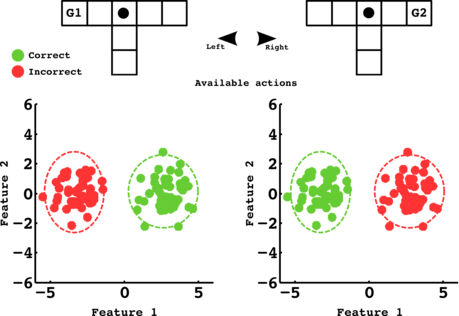
\includegraphics[width=\twotworldsize\columnwidth]{\visualspdf/tuto_feedback/Tworld_feedback_labeled_right_left_with_gaussian.pdf}
  \caption{Result of the labeling process if the agent only performs right and left actions in the top of the T world. This is the symmetry problem encountered in previous chapter~\ref{chapter:lfui:symmetries}. The resulting signal-label pairs for G1 and G2, while symmetric, are both as likely to explain the data.}
  \label{fig:planningrightleft}
\end{figure}

Considering that the agent does not know the signal to meaning mapping, a sensitive option is to select actions unequivocally identifying the signal model. In the T world, taking only up and down actions in the trunk of the T leads to identical interpretation for each hypothesis (see Figure~\ref{fig:planningupdown}). However this action selection method alone does not allow to disambiguate between hypothesis as both model are the same, therefore as valid. Moreover, in most settings, such as the grid world we consider later, there is no state-action pair leading to unequivocal interpretation of the signals.

\begin{figure}[!htbp]
  \centering
  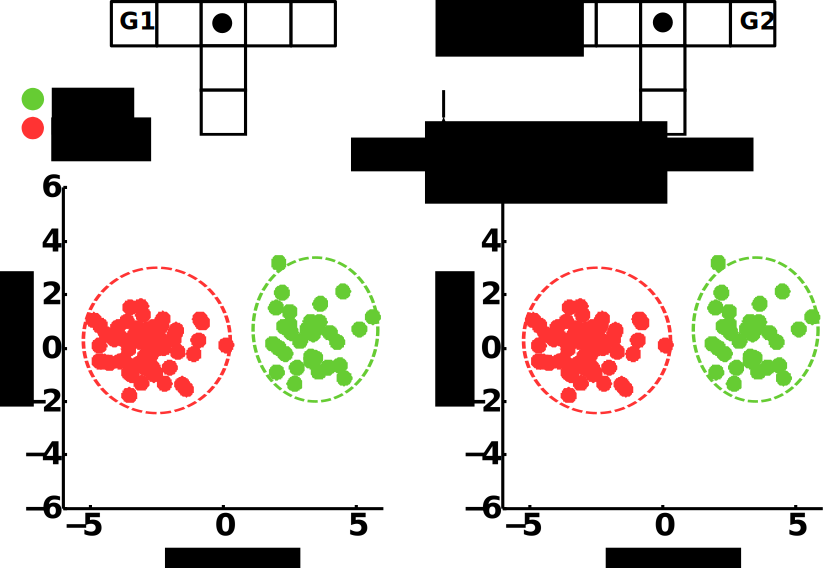
\includegraphics[width=\twotworldsize\columnwidth]{\visualspdf/tuto_feedback/Tworld_feedback_labeled_up_down_with_gaussian.pdf}
  \caption{Result of the labeling process if the agent only performs up and down actions in the trunk of the T. The interpretation of the signals are the same for both hypothesis, therefore as likely to explain the data.}
  \label{fig:planningupdown}
\end{figure}

Those two examples exemplify the specificity of the uncertainty in our problem. The agent can not just try to differentiate hypothesis by finding state-action pairs where expected feedback differs (left-right actions in Figure~\ref{fig:planningrightleft}) but should also collect data to build a good model (up-down actions in Figure~\ref{fig:planningupdown}). What is the optimal next action to take in the previous condition?

\begin{itemize}
\item In the situation of Figure~\ref{fig:planningrightleft}, the agent ends-up with a symmetric interpretation for G1 and G2 and it should therefore perform an action breaking this symmetry. It must collect one signal whose label is  identical for both hypothesis. Performing a ``down'' action in the T trunk, both hypothesis will associate an ``incorrect'' label to the received signal, which will break the symmetry.
\item In the situation of Figure~\ref{fig:planningupdown}, the agent ends-up with an identical interpretation for G1 and G2 and it should therefore collects one signal whose label is different for each hypothesis. By performing a ``left'' action in the top of the T, hypothesis G1 will associate the label ``correct'', while hypothesis G2 will associate the label ``incorrect'', which will break the similarity between models.
\end{itemize}

Can we find an uncertainty measure that account for both cases? The measure defined in the previous section would not work because it was independent of the signal-to-meaning mapping. Indeed, this mapping was the same for every hypothesis, but in this work, each hypothesis has a different signal-to-meaning mapping. In other words, there is an additional layer of uncertainty on the signal-to-meaning mapping.

% \begin{itemize}
% \item In the situation from Figure~\ref{fig:planningrightleft}, when going left both hypothesis agree that they will receive a signal in the right part of the feature space even if they disagree on its meaning. However for action down, both hypothesis agree they should receive a signal of meaning ``incorrect'' but disagree on the expected location of such signal in the feature space.
% \item In the situation from Figure~\ref{fig:planningupdown}, when going down both hypothesis agree they will receive a signal in the left part of the feature space and agree on its meaning. However for action left, both hypothesis disagree about the meaning of the signal they should receive and as both share the same signal model they expect a signal in different locations of the feature space.
% \end{itemize}

We must therefore measure uncertainty taking into account the uncertainty related to both the different tasks and different classifiers. This process will be exemplified in the next section using our T world example. We will present two ways of measuring the uncertainty. The first method measures the uncertainty on the expected signals between each hypothesis. The second method measures uncertainty on the meaning space by making hypothesis on future observed signals.

%%%%%%%%%%%%%%%%%%%%%%%%%%%%%%%%%%%%%%%%%%%%%%
%%%%%%%%%%%%%%%%%%%%%%%%%%%%%%%%%%%%%%%%%%%%%%
%%%%%%%%%%%%%%%%%%%%%%%%%%%%%%%%%%%%%%%%%%%%%%
%%%%%%%%%%%%%%%%%%%%%%%%%%%%%%%%%%%%%%%%%%%%%%
%%%%%%%%%%%%%%%%%%%%%%%%%%%%%%%%%%%%%%%%%%%%%%
\section{How can we measure the uncertainty}
\label{chapter:planning:how}

Before providing visual examples and equations of our uncertainty measures, we remind the importance of weighting the votes of each hypothesis proportionally to their current probability. We then present our two methods. The first method measures the uncertainty on the expected signals between each hypothesis. The second method measures uncertainty on the meaning space by making hypothesis on future observed signals.

\subsection{The importance of weighting}

We want to measure the uncertainty about both the tasks and signal models in order to collect information allowing to reduce this uncertainty. The uncertainty is therefore not constant, it depends on our current belief about each hypothesis and must be updated when new teaching signals are observed.

As we want to find which task is the correct one among the set of task hypothesis, our aim is to pull apart the hypotheses that are currently the more probable. Once we have ruled out half of the hypotheses, we should only focus on differentiating the remaining hypotheses. Therefore, when estimating the uncertainty, we should weight each vote according to each hypothesis probability. In practice, if one hypothesis has a probability of 1 (i.e. all other hypotheses have a probability of zero) there should be no uncertainty for all state-action pairs.

\subsection{A measure on the signal space}
\label{chapter:planning:uncertaintysignalspace}

As explained in section~\ref{chapter:planning:where}, our uncertainty measure should take into account both the uncertainty due to the task and the signal model. We illustrate how this uncertainty can be measured by comparing the expected signals from each task hypothesis.

\subsubsection*{Symmetric signal models}

We start by considering the situation of Figure~\ref{fig:planningrightleft} where G1 and G2 have symmetric signal models. As depicted in Figure~\ref{fig:uncertaintysignalrightleftagree}, when selecting action left, both hypothesis agree that they should receive a signal in the right part of the feature space, even if they disagree on its meaning. Therefore taking action left in state 3 has low uncertainty on the expected signal.

\begin{figure}[!htbp]
  \centering
  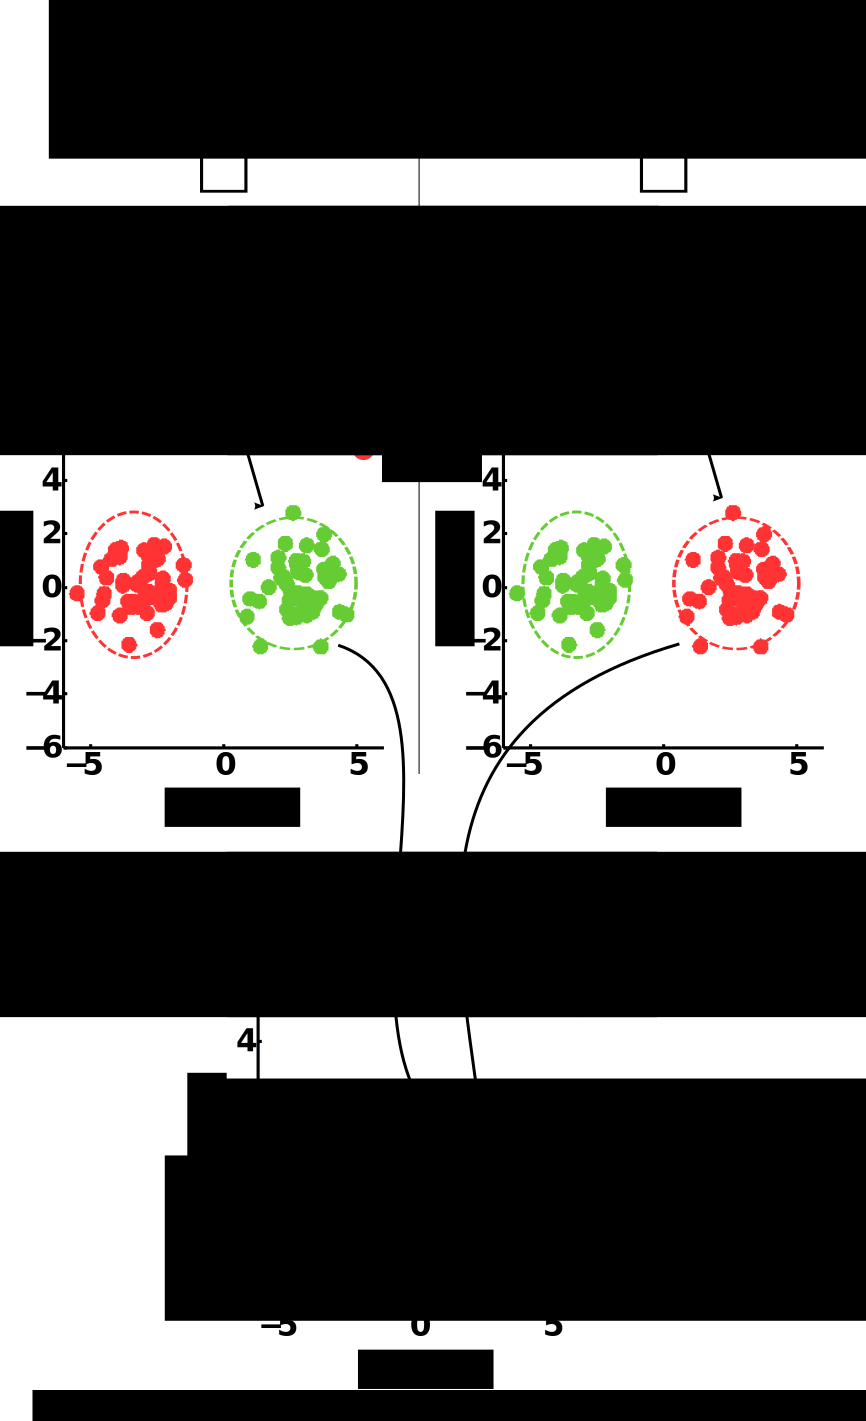
\includegraphics[width=\twoplanningwidth\columnwidth]{\visualspdf/planning/planning_right_left_agree.pdf}
  \caption{Expected signal for both hypothesis if agent performs action left in state 3 and given they currently have a symmetric interpretation of the signals (see Figure~\ref{fig:planningrightleft}). Both hypotheses expect the same signal, therefore there is no uncertainty associated to this state-action pair, and the agent should not select this action.}
  \label{fig:uncertaintysignalrightleftagree}
\end{figure}

However for action down, both hypothesis agree they should receive a signal of meaning ``incorrect'', but disagree on the expected location of such signal in the feature space (see Figure~\ref{fig:uncertaintysignalrightleftdisagree}). Therefore taking action down in state 3 has high uncertainty on the expected signal.

\begin{figure}[!htbp]
  \centering
  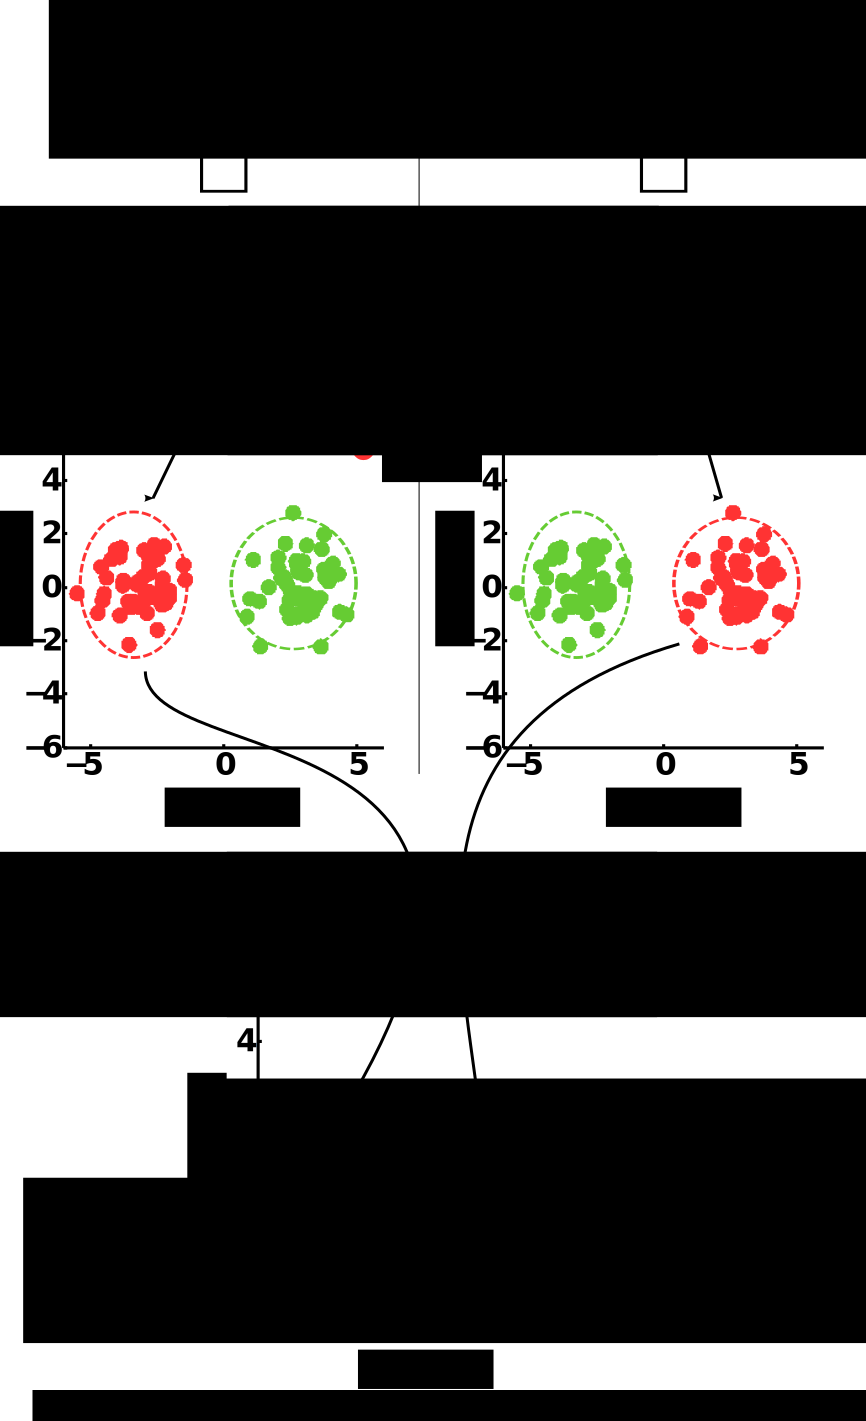
\includegraphics[width=\twoplanningwidth\columnwidth]{\visualspdf/planning/planning_right_left_disagree.pdf}
  \caption{Expected signal for both hypothesis if agent performs action down in state 3 and given they currently have a symmetric interpretation of the signals (see Figure~\ref{fig:planningrightleft}). The two hypotheses expect two different signals, therefore there is high uncertainty associated to this state-action pair, and the agent should better perform this action.}
  \label{fig:uncertaintysignalrightleftdisagree}
\end{figure}

\subsubsection*{Identical signal models}

We now consider the situation of Figure~\ref{fig:planningupdown} where G1 and G2 have the same signal model. As depicted in Figure~\ref{fig:uncertaintysignalupdownagree}, when going down both hypothesis agree that they should receive a signal in the left part of the feature space, and agree on its meaning. Therefore taking action down in state 3 has low uncertainty on the expected signal.

\begin{figure}[!htbp]
  \centering
  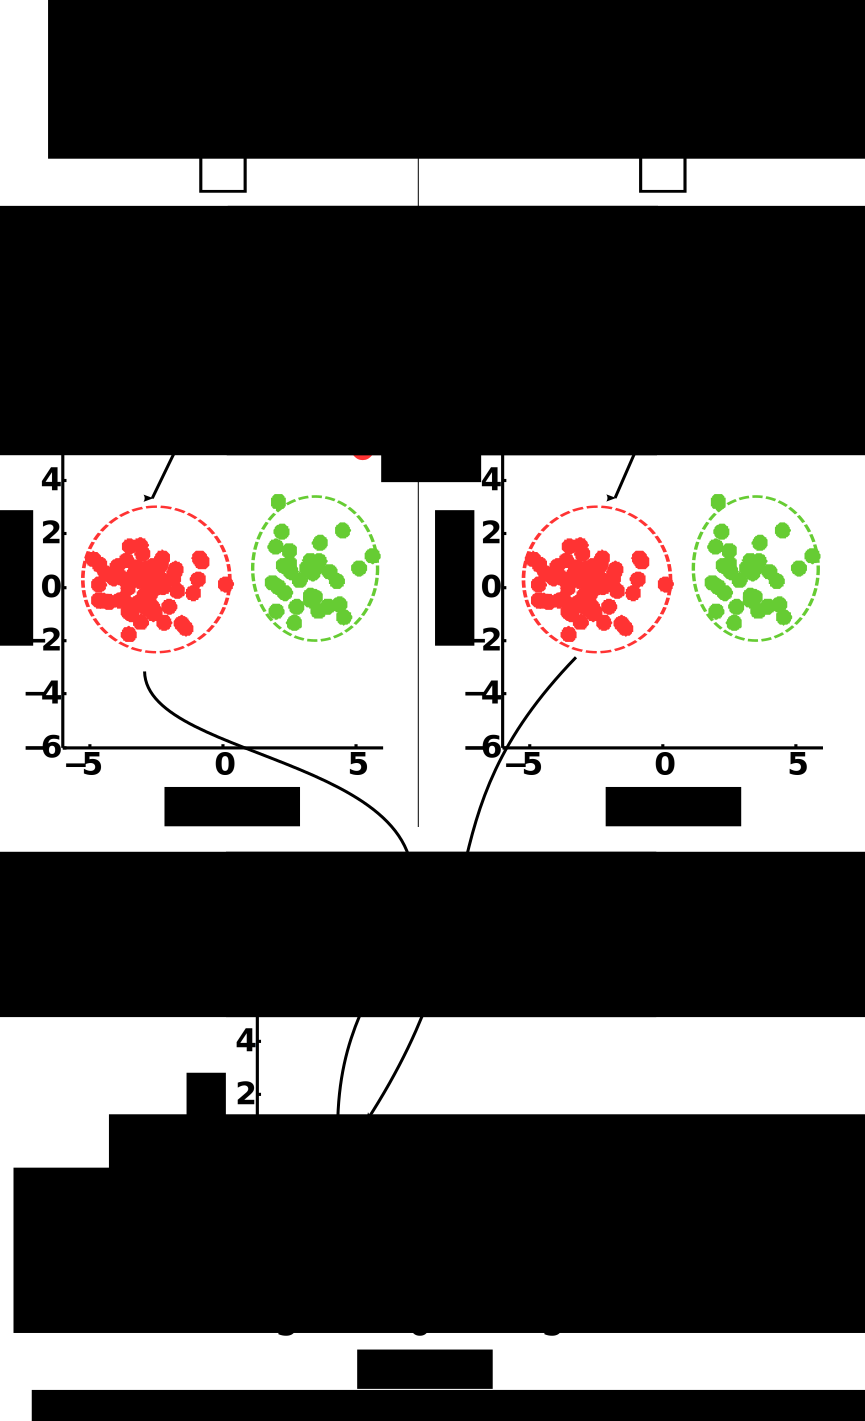
\includegraphics[width=\twoplanningwidth\columnwidth]{\visualspdf/planning/planning_up_down_agree.pdf}
  \caption{Expected signal for both hypothesis if agent performs action down in state 3 and given they currently have a similar interpretation of the signals (see Figure~\ref{fig:planningupdown}). Both hypothesis expect the same signal, therefore there is no uncertainty associated to this state-action pair, and the agent should not select this action.}
  \label{fig:uncertaintysignalupdownagree}
\end{figure}

However for action left, both hypothesis disagree about the meaning of the signal they should receive, and, as both share the same signal model, they expect a signal in different locations of the feature space (see Figure~\ref{fig:uncertaintysignalupdowndisagree}). Therefore taking action left in state 3 has high uncertainty on the expected signal.

\begin{figure}[!htbp]
  \centering
  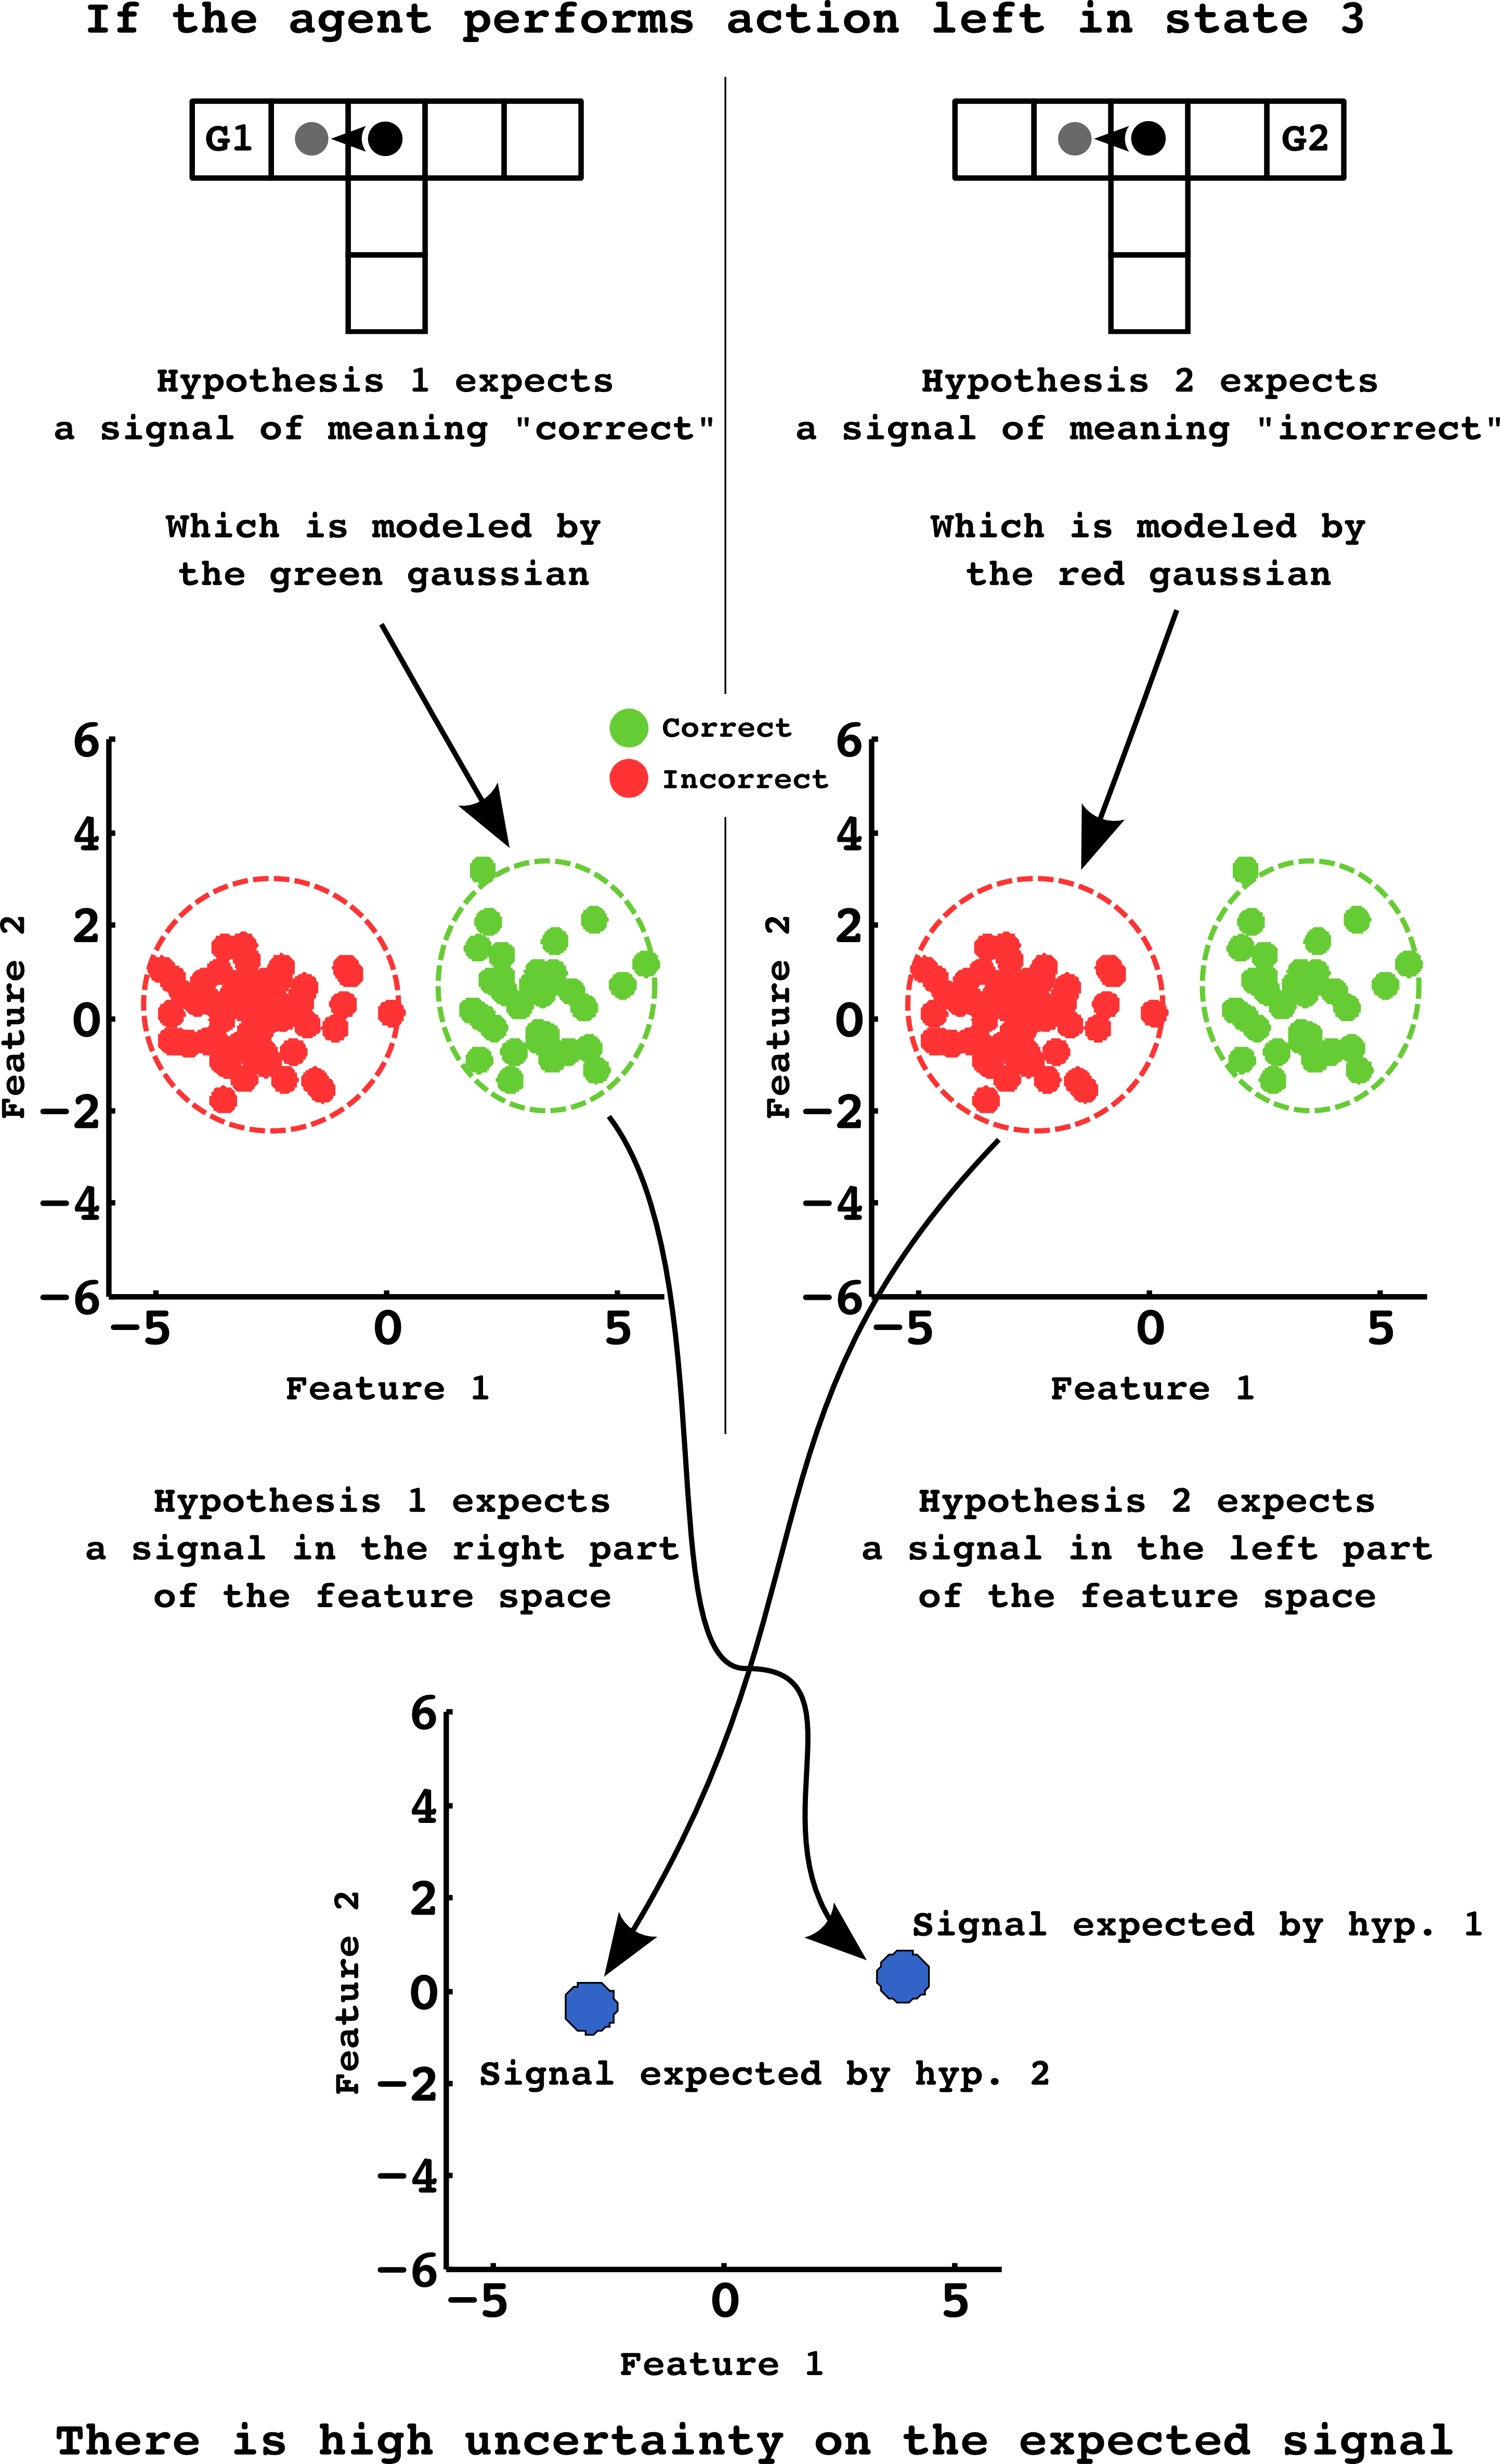
\includegraphics[width=\twoplanningwidth\columnwidth]{\visualspdf/planning/planning_up_down_disagree.pdf}
  \caption{Expected signal for both hypothesis if agent performs action left in state 3 and given they currently have a similar interpretation of the signals (see Figure~\ref{fig:planningupdown}). The two hypothesis expect two different signals, therefore there is high uncertainty associated to this state-action pair, and the agent should better perform this action.}
  \label{fig:uncertaintysignalupdowndisagree}
\end{figure}


\subsubsection*{Equations}

To sum up, to compute the uncertainty associated to a state-action pair, we can compute the similarity between the expected signals from each task. The more the expected signals are similar the less there is uncertainty. And we remind that the vote of a hypothesis should be weighted by the current probability of this hypothesis.

% a state-action pair where the optimal actions and the signal models are the same for all hypotheses wont help discriminating hypotheses. It will be less informative that any other state-action where either optimal actions or signal models differ between hypotheses. 

Our visual examples represent the expected signal for each hypothesis as the mean of the signal distribution corresponding to the expected label. This is a very rough approximation, indeed, the signals are modeled by a Gaussian distribution. Therefore comparing the similarity between the respective distribution would be more suited than comparing only their mean. Moreover, the frame function is not always deterministic. For example, we take into account possible teaching mistakes by assigning some probability of receiving an ``incorrect'' feedback while the action was optimal. Ideally, this should also be taken into account when computing the similarity between signal distributions. In addition, our examples consider only two hypotheses, and as soon as the number of hypotheses increases, we should compute the similarity between a multitude of distributions. 

Measuring similarity between expected signals can be complex. In practice, it will be easier and more efficient to compute the uncertainty based on the mean of the distribution only. Whatever the method chosen, we define a similarity matrix $S$ where each element $S_{ij}(s,a)$ corresponds to the similarity between the expected signals from tasks $i$ and task $j$ if action $a$ is performed in state $s$.

% which should in this example composed of mixture of Gaussian whose associated weight are the probability of receiving their associated meaning. 

The final uncertainty value $U(s,a)$ is computed as the opposite of the weighted sum of the similarity matrix elements:

\begin{eqnarray}
U(s,a) &=& - \sum_{i = 1}^{T} \sum_{j = 1}^{T} ~~ S_{ij}(s,a) ~ p(\xi_i) ~ p(\xi_j)
\end{eqnarray}

% We define a measure of global uncertainty $U(s,a)$ that is higher when, for a given state-action, there is a high incongruity between either optimal actions or signal models. 

Computed for every state and action, this measure is then used as an exploration bonus to guide the agent towards states that better disambiguate task hypotheses. We provide an example of planning using this method in chapter~\ref{chapter:limitations:overlap}, where we measure similarity between Gaussian distribution using their means only.

\subsection{A measure projected in the meaning space}
\label{chapter:planning:uncertiantyprojected}

Estimating uncertainty in the signal space can be very costly. It requires to compute, for every state-action pair, the overlap between many continuous probability distributions weighted by their respective expected contributions. In this subsection we present another metric for computing the uncertainty which relies on our pseudo-likelihood measure defined in chapter~\ref{chapter:lfui:how}. This method relies on sampling some teaching signals and asking every hypothesis whether the sampled signals are expected or not given a state-action pair.

\subsubsection*{Symmetric signal models}

We start by considering the situation of Figure~\ref{fig:planningrightleft} where the two hypothesis have symmetric signal models. As depicted in Figure~\ref{fig:uncertaintymeaningrightleftexpectedleft}, when selecting action left in state 3 and if the user sends a signal in the right part of the feature space, both hypothesis agree that this particular signal is expected given this state-action pair. Hypothesis 1 expects a signal of meaning ``correct'', and the teacher signal is classified as being of class ``correct''. Hypothesis 2 expects a signal of meaning ``incorrect'' and the teacher signal is classified as being of class ``incorrect''. Therefore receiving this particular signal after taking action left in state 3 has low uncertainty.

\begin{figure}[!htbp]
  \centering
  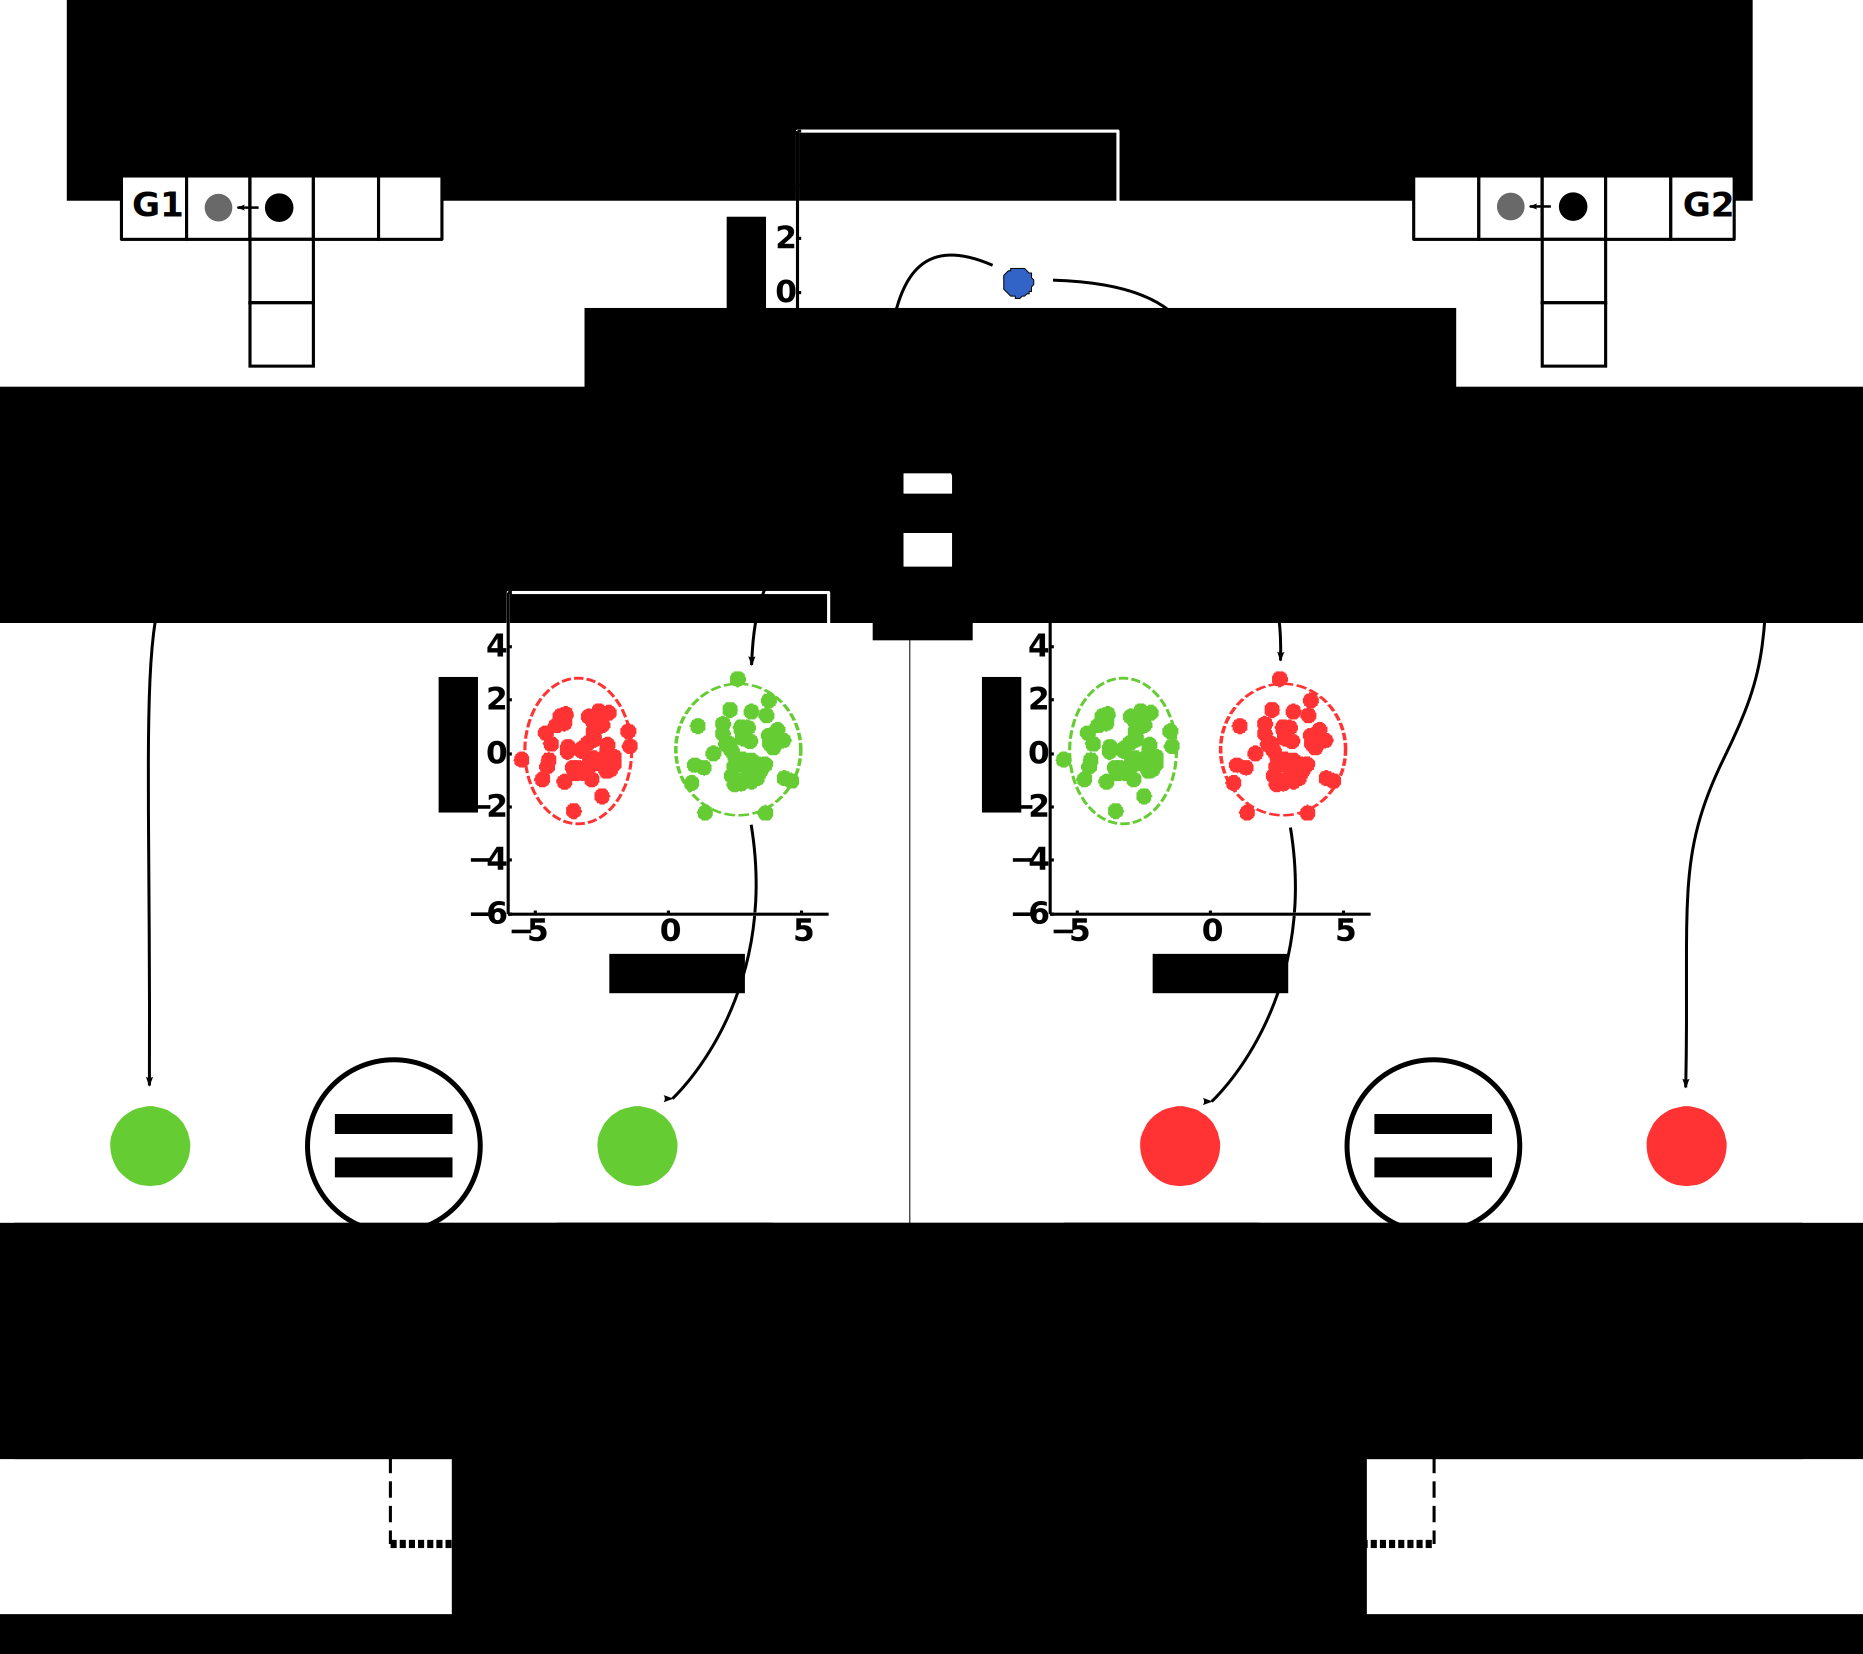
\includegraphics[width=\threeplanningwidth\columnwidth]{\visualspdf/planning/planning_right_left_expected_matched.pdf}
  \caption{Matching between expected labels and the prediction of a teaching signal sampled on the right side of the feature space and if the agent performs action left in state 3 and the two hypothesis currently have a symmetric interpretation of the signals (see Figure~\ref{fig:planningrightleft}). Both hypothesis agree that the label associated to a signal on the right side of the feature space matches with the label predicted given the frame and the state-action pair considered. Therefore, there is no uncertainty associated to this state-action pair and the agent should not select action left.}
  \label{fig:uncertaintymeaningrightleftexpectedleft}
\end{figure}

This same process can be executed for any teaching signal. For example, as depicted in Figure~\ref{fig:uncertaintymeaningrightleftexpectedright}, considering a teaching signal on the left side of the feature space, if the agent performs action left in state 3, both hypothesis agree that this particular signal is not expected. Hypothesis 1 expects a signal of meaning ``correct'', and the teacher signal is classified as being of class ``incorrect''. Hypothesis 2 expects a signal of meaning ``incorrect'' and the teacher signal is classified as being of class ``correct''. Therefore receiving this particular signal after taking action left in state 3 has low uncertainty.

\begin{figure}[!htbp]
  \centering
  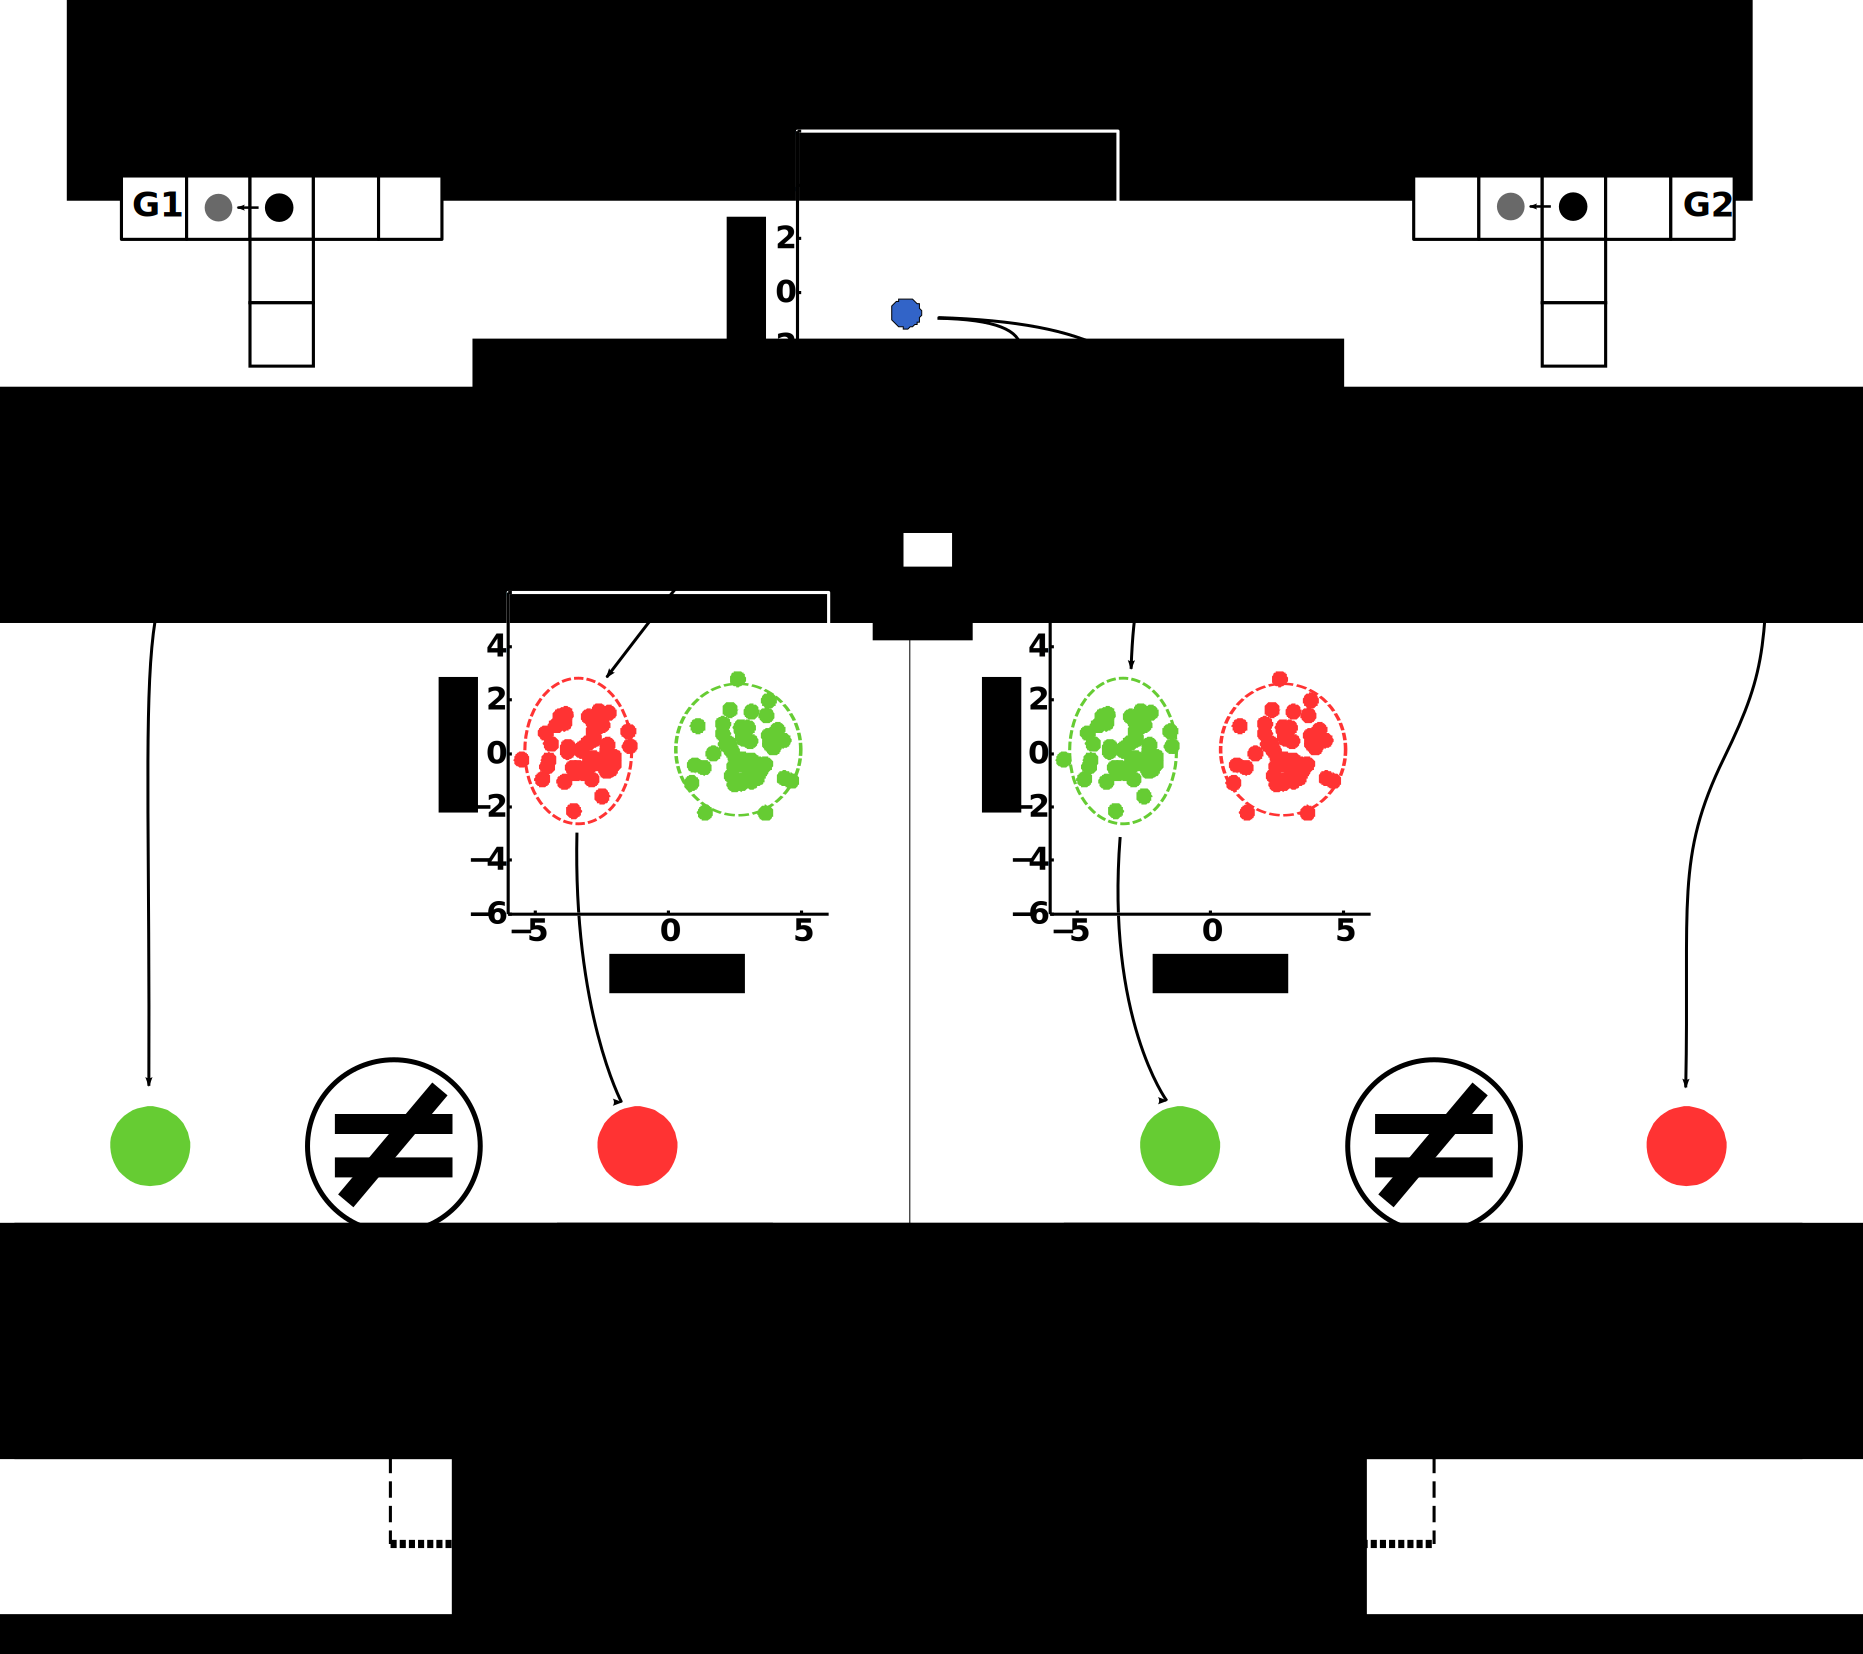
\includegraphics[width=\threeplanningwidth\columnwidth]{\visualspdf/planning/planning_right_left_expected_unmatched.pdf}
  \caption{Matching between expected labels and the prediction of a teaching signal sampled on the left side of the feature space for the two hypothesis if the agent performs action left in state 3 and the two hypothesis currently have a symmetric interpretation of the signals (see Figure~\ref{fig:planningrightleft}). Both hypothesis agree that the label associated to a signal on the left side of the feature space does not match with the label predicted given the frame and the state-action pair considered. Therefore, there is no uncertainty associated to this state-action pair and the agent should not select action left.}
  \label{fig:uncertaintymeaningrightleftexpectedright}
\end{figure}

However for action down, the two hypothesis disagree on whether such signals are expected or not given the state-action pair considered. As depicted in Figure~\ref{fig:uncertaintymeaningrightleftunexpectedright}, when selecting action down in state 3 and if the user sends a signal in the right part of the feature space, hypothesis 1 expects a signal of meaning ``incorrect'', and the teacher signal is classified as being of class ``correct''. And hypothesis 2 expects a signal of meaning ``incorrect'' and the teacher signal is classified as being of class ``incorrect''. Therefore receiving this particular signal after taking action down in state 3 is not expected for hypothesis 1 but expected for hypothesis 2, there is high uncertainty.

\begin{figure}[!htbp]
  \centering
  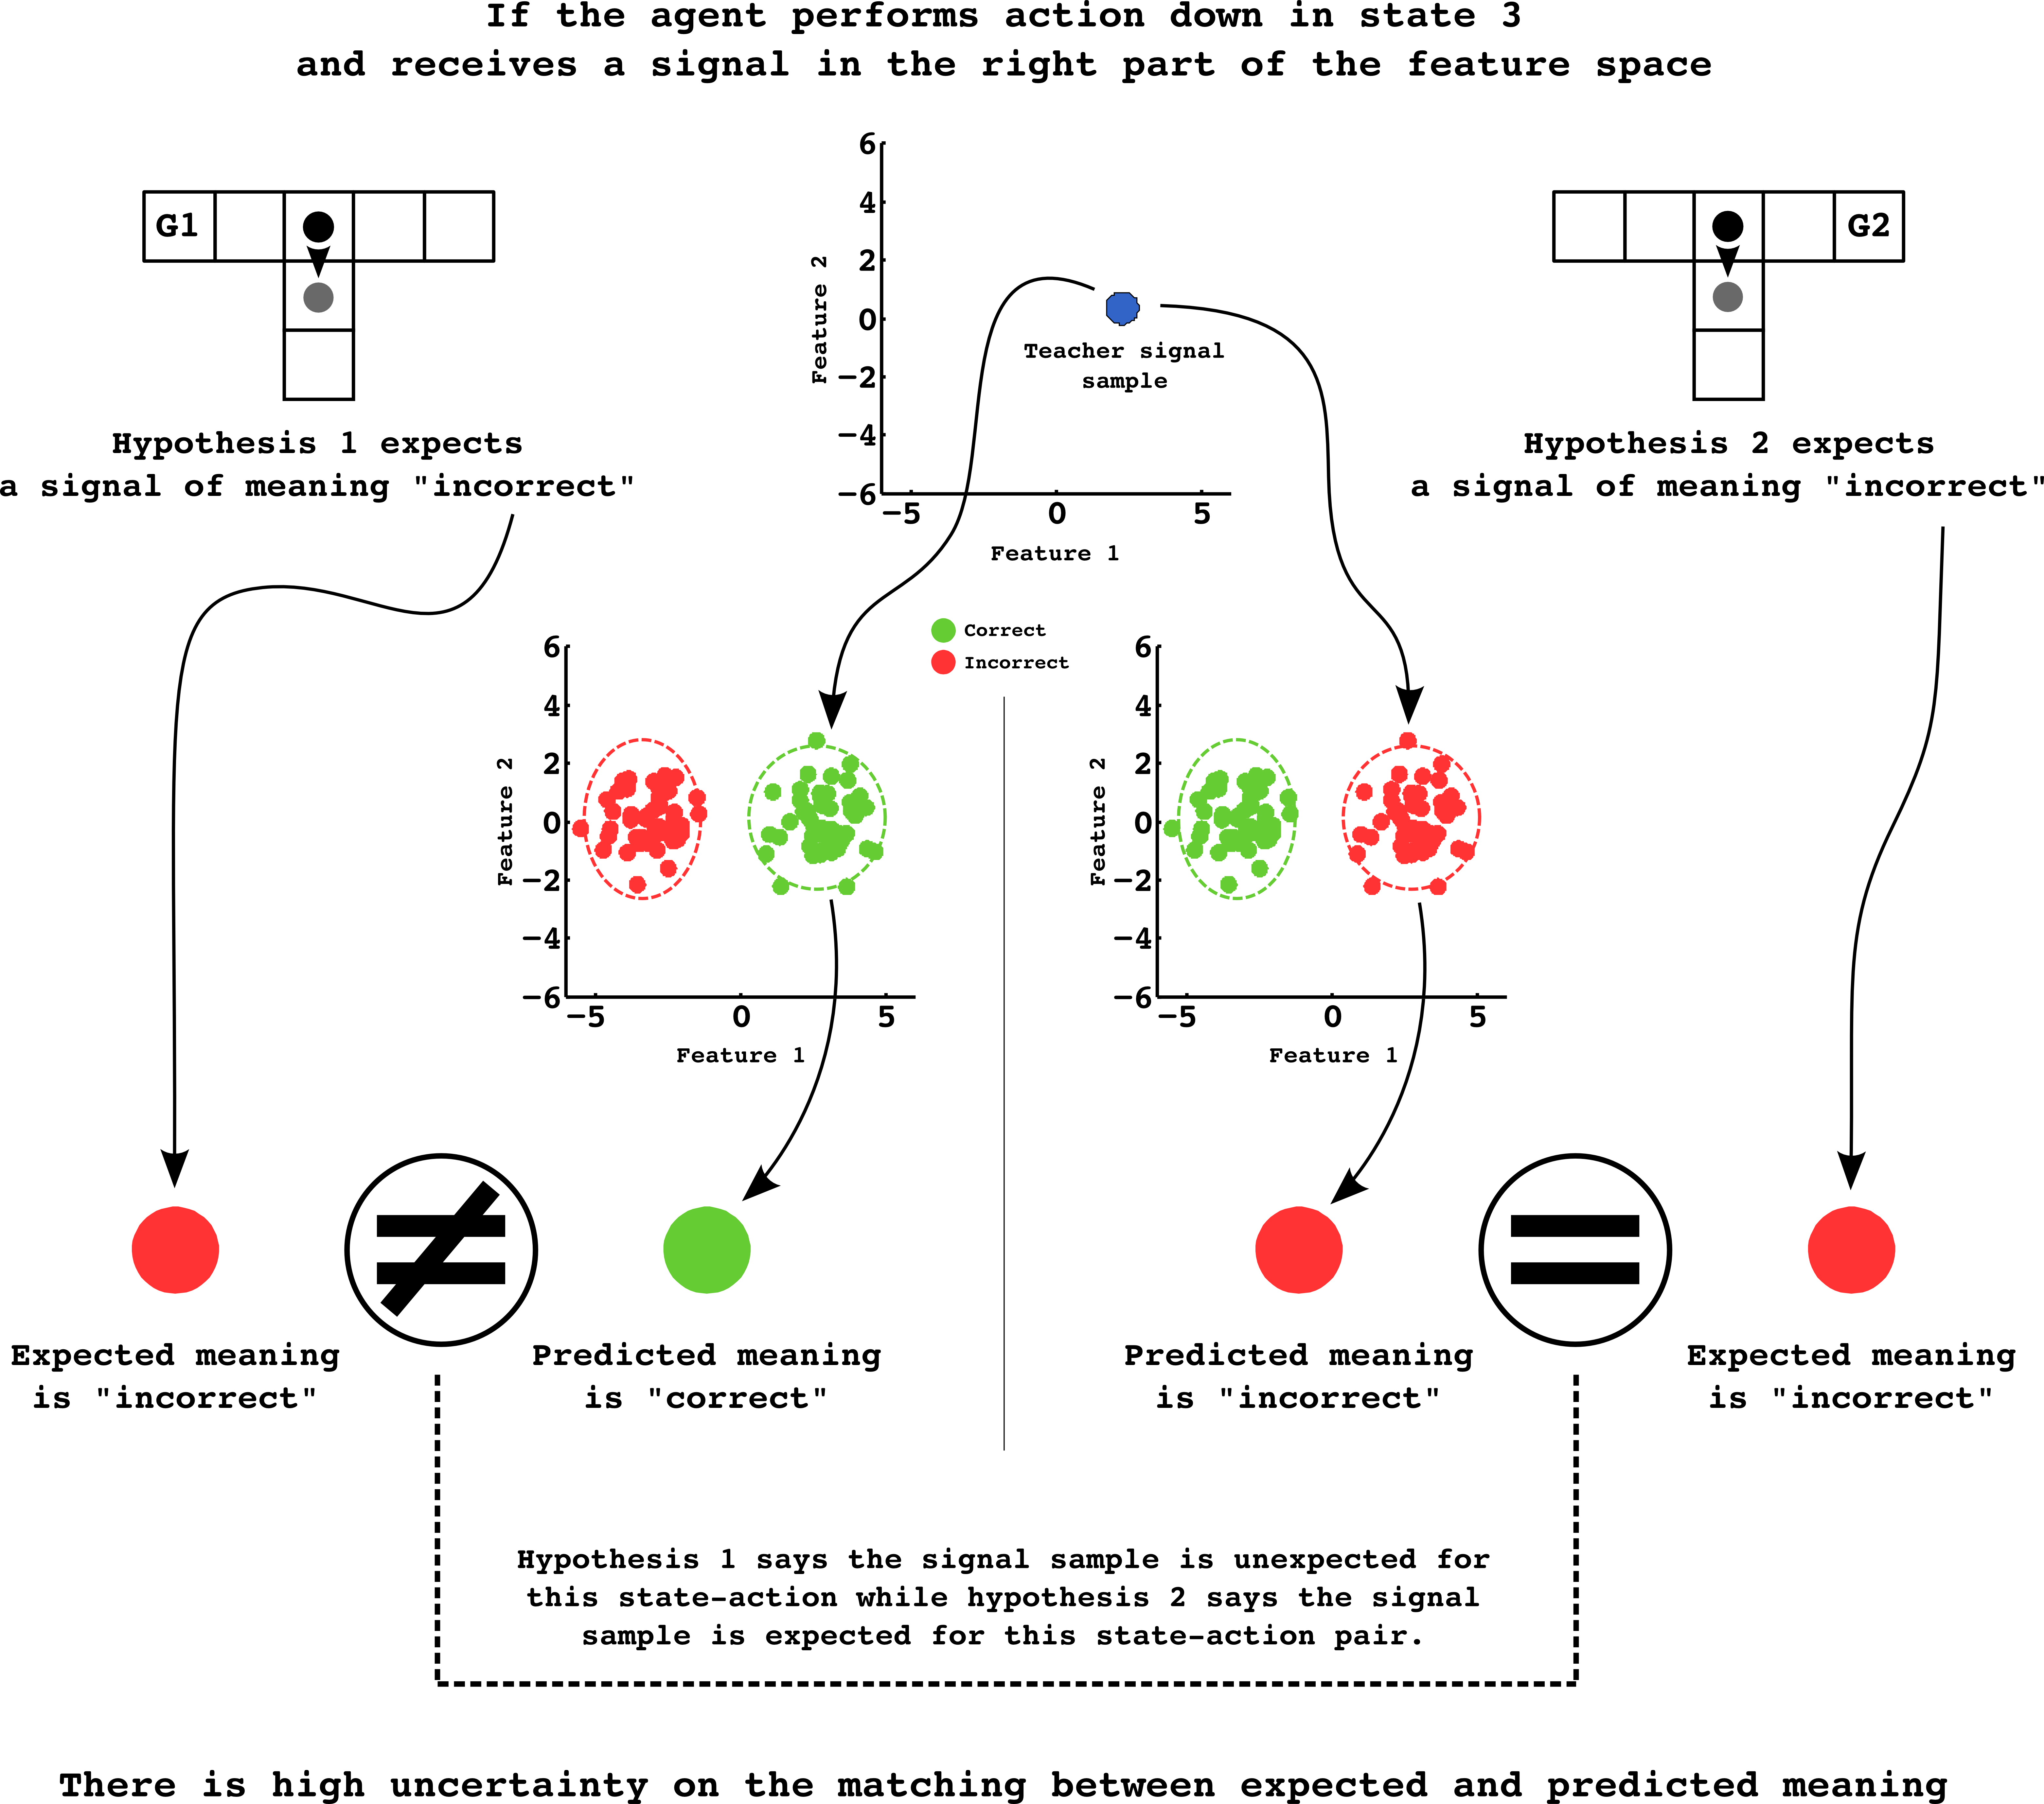
\includegraphics[width=\threeplanningwidth\columnwidth]{\visualspdf/planning/planning_right_left_unexpected_right_signal.pdf}
  \caption{Matching between expected labels and the prediction of a teaching signal sampled on the right side of the feature space for the two hypothesis if the agent performs action down in state 3 and the two hypothesis currently have a symmetric interpretation of the signals (see Figure~\ref{fig:planningrightleft}). Hypothesis 1 says a signal on the right side of the feature space means ``correct'' which was not expected given the interaction frame, while hypothesis 2 expected a signal meaning ``incorrect'' and classify the signal as ``incorrect'' which is what was expected. Therefore there is high uncertainty associated to this state-action pair and the agent should better perform action down in order to disambiguate between hypothesis.}
  \label{fig:uncertaintymeaningrightleftunexpectedright}
\end{figure}

Similarly, as depicted in Figure~\ref{fig:uncertaintymeaningrightleftunexpectedleft}, considering a teaching signal on the left side of the feature space, if the agent performs action down in state 3, hypothesis 1 expects a signal of meaning ``incorrect'', and the teacher signal is classified as being of class ``incorrect''. And hypothesis 2 expects a signal of meaning ``incorrect'' and the teacher signal is classified as being of class ``correct''. Therefore receiving this particular signal after taking action down in state 3 is expected for hypothesis 1 but not expected for hypothesis 2, there is high uncertainty.

\begin{figure}[!htbp]
  \centering
  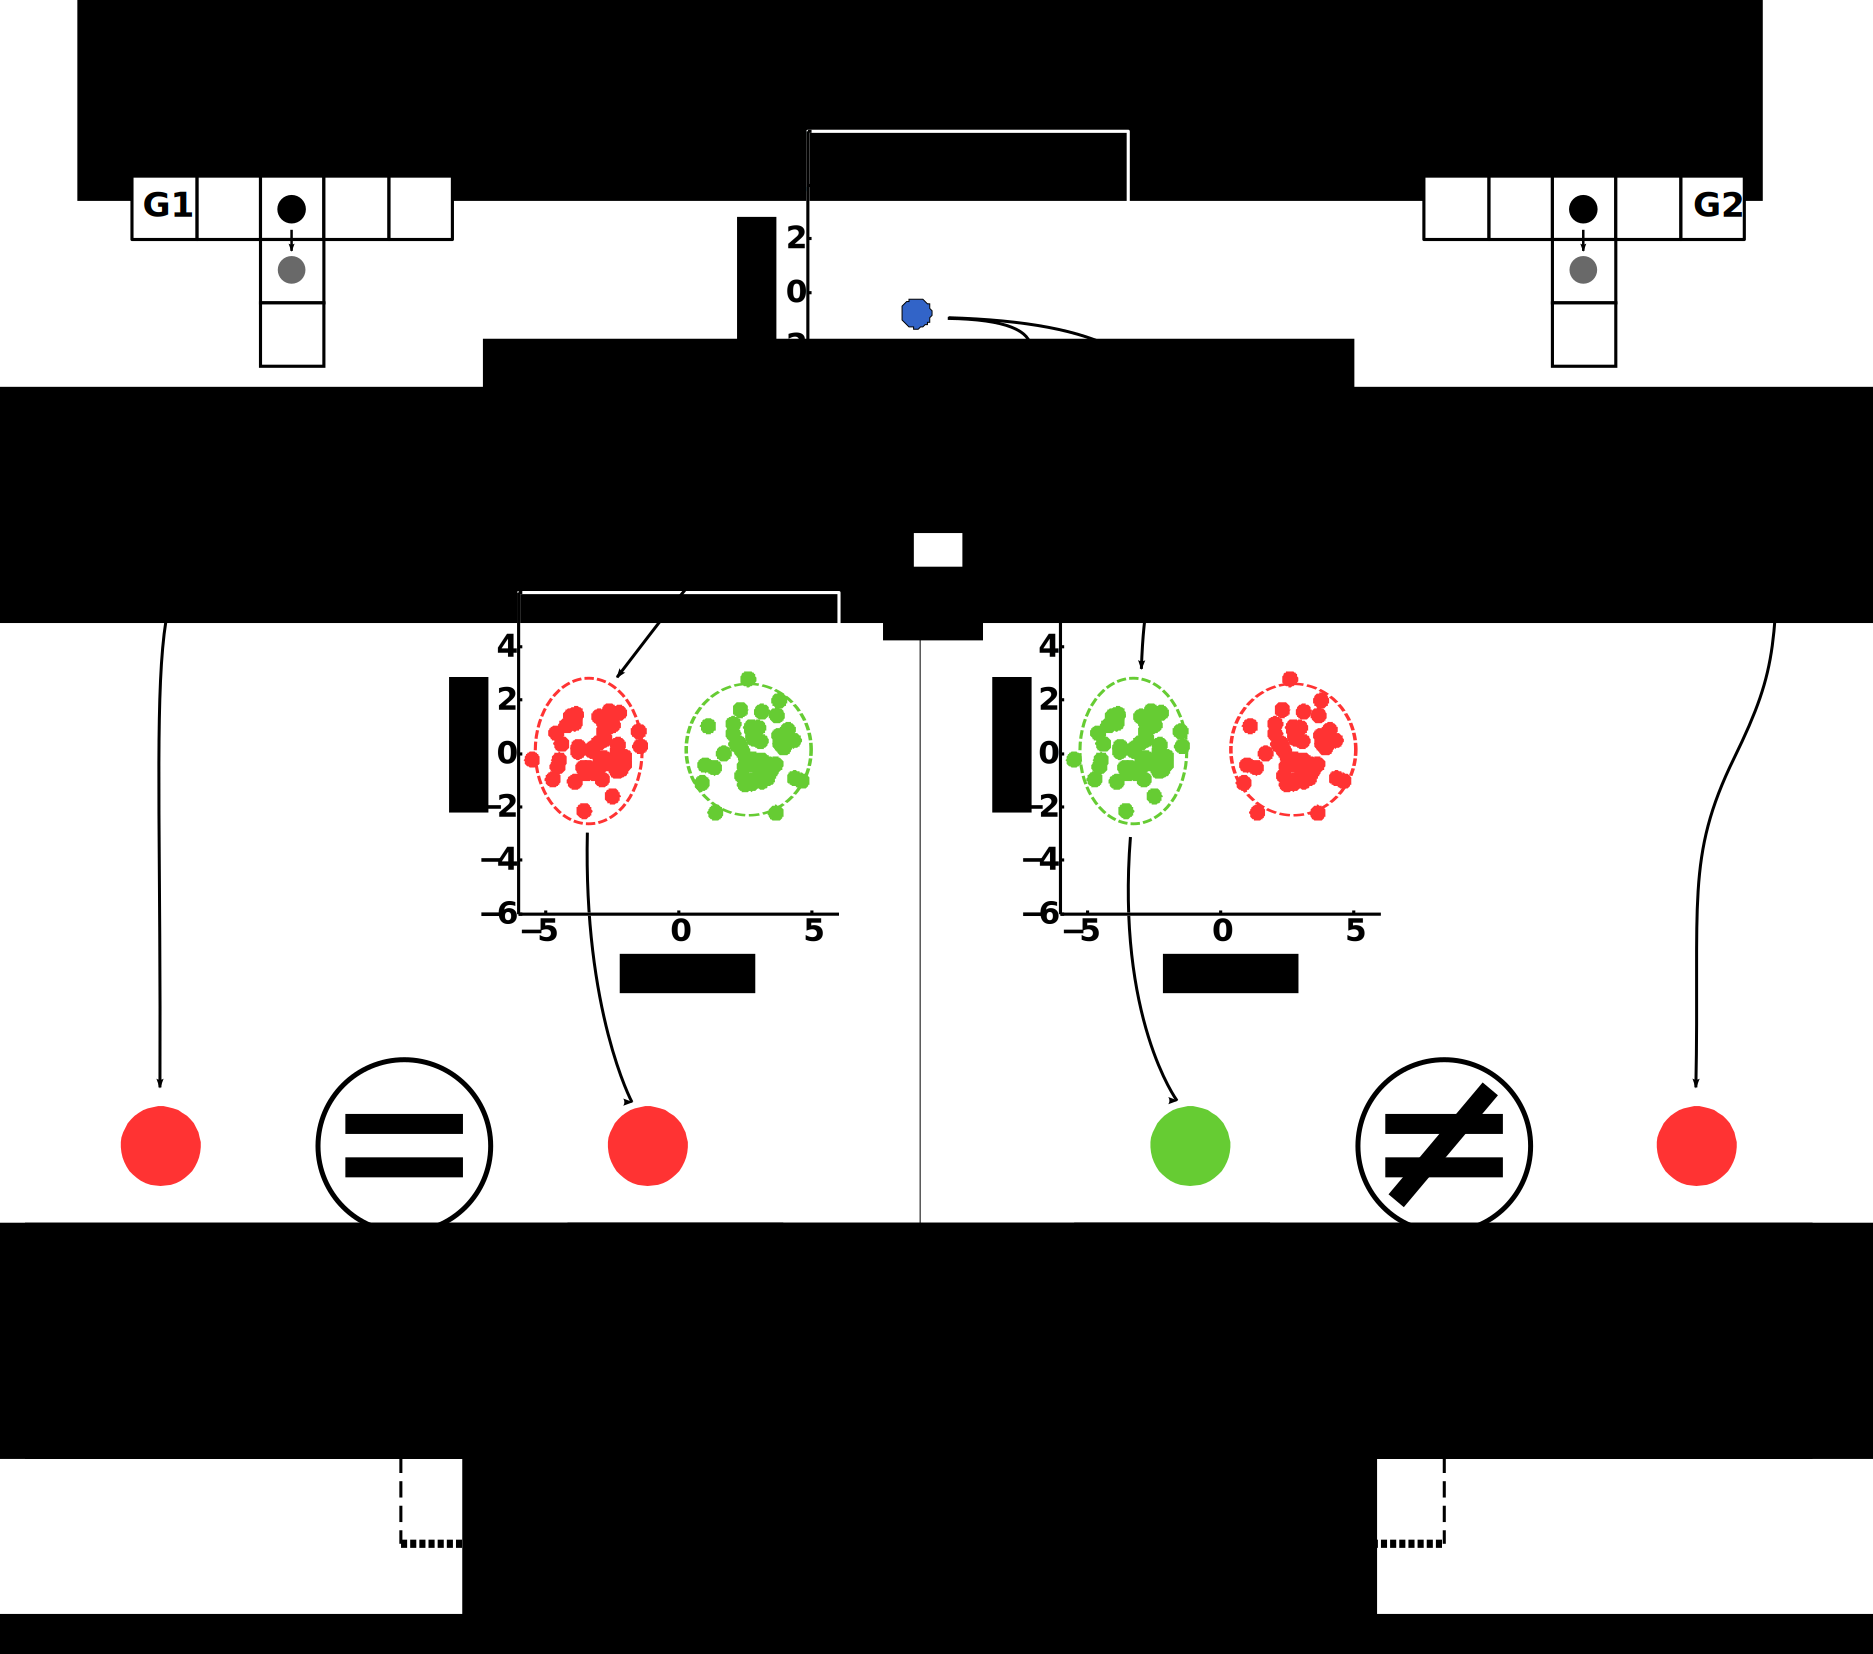
\includegraphics[width=\threeplanningwidth\columnwidth]{\visualspdf/planning/planning_right_left_unexpected_left_signal.pdf}
  \caption{Matching between expected labels and the prediction of a teaching signal sampled on the left side of the feature space for the two hypothesis if the agent performs action down in state 3 and the two hypothesis currently have a symmetric interpretation of the signals (see Figure~\ref{fig:planningrightleft}). Hypothesis 1 says a signal on the left side of the feature space means ``incorrect'' which was expected given the interaction frame, while hypothesis 2 expected a signal meaning ``incorrect'' but classify the signal as ``correct'' which was not expected. Therefore there is high uncertainty associated to this state-action pair and the agent should better perform action down in order to disambiguate between hypothesis..}
  \label{fig:uncertaintymeaningrightleftunexpectedleft}
\end{figure}

\subsubsection*{Identical signal models}

We now consider the situation of Figure~\ref{fig:planningupdown} when the same model is shared between hypothesis. As depicted in Figure~\ref{fig:uncertaintymeaningupdownexpectedright}, when selecting action down in state 3 and if the user sends a signal in the right part of the feature space, both hypothesis agree that this particular signal is unexpected given this state-action pair. Hypothesis 1 expects a signal of meaning ``incorrect'', and the teacher signal is classified as being of class ``correct''. Hypothesis 2 expects a signal of meaning ``incorrect'' and the teacher signal is classified as being of class ``correct''. Therefore receiving this particular signal after taking action down in state 3 has low uncertainty.

\begin{figure}[!htbp]
  \centering
  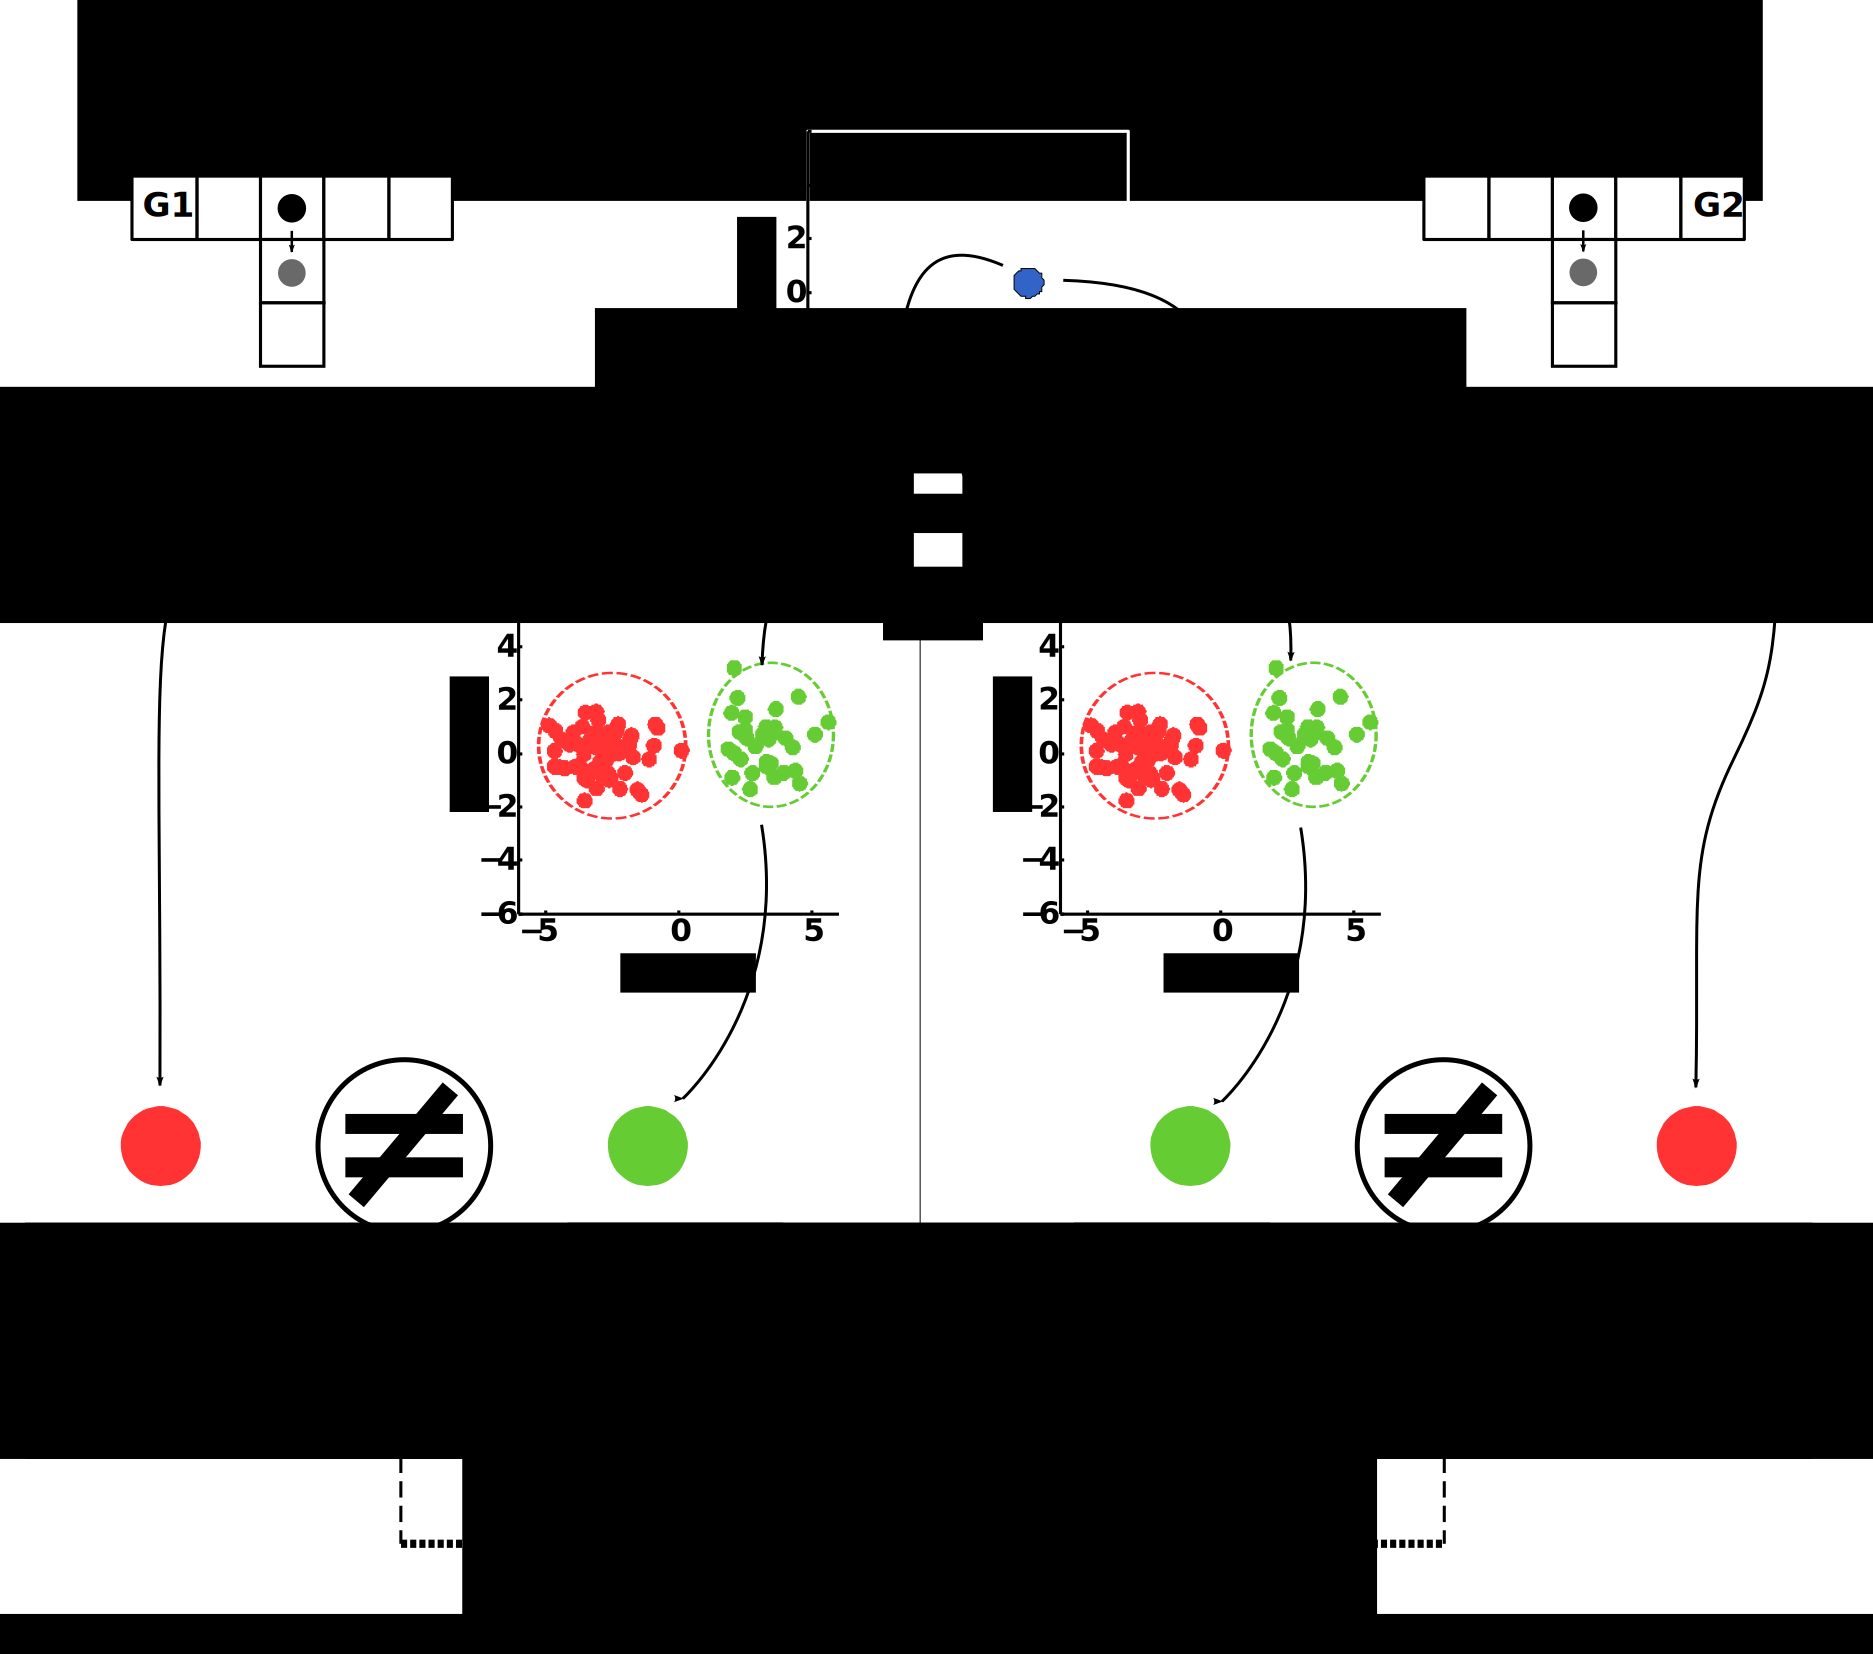
\includegraphics[width=\threeplanningwidth\columnwidth]{\visualspdf/planning/planning_up_down_expected_unmatched.pdf}
  \caption{Matching between expected labels and the prediction of a teaching signal sampled on the right side of the feature space for the two hypothesis if the agent performs action down in state 3 and the two hypothesis currently have a symmetric interpretation of the signals (see Figure~\ref{fig:planningupdown}). Both hypothesis agree that the label associated to a signal on the right side of the feature space does not match with the label predicted given the frame and the state-action pair considered. Therefore there is no uncertainty associated to this state-action pair and the agent should not select action down.}
  \label{fig:uncertaintymeaningupdownexpectedright}
\end{figure}

This same process can be executed for any teaching signal. For example, as depicted in Figure~\ref{fig:uncertaintymeaningupdownexpectedleft}, considering a teaching signal on the left side of the feature space, if the agent performs action down in state 3, both hypothesis agree that this particular signal is expected. Hypothesis 1 expects a signal of meaning ``incorrect'', and the teacher signal is classified as being of class ``incorrect''. Hypothesis 2 expects a signal of meaning ``incorrect'' and the teacher signal is classified as being of class ``incorrect''. Therefore receiving this particular signal after taking action down in state 3 has low uncertainty.

\begin{figure}[!htbp]
  \centering
  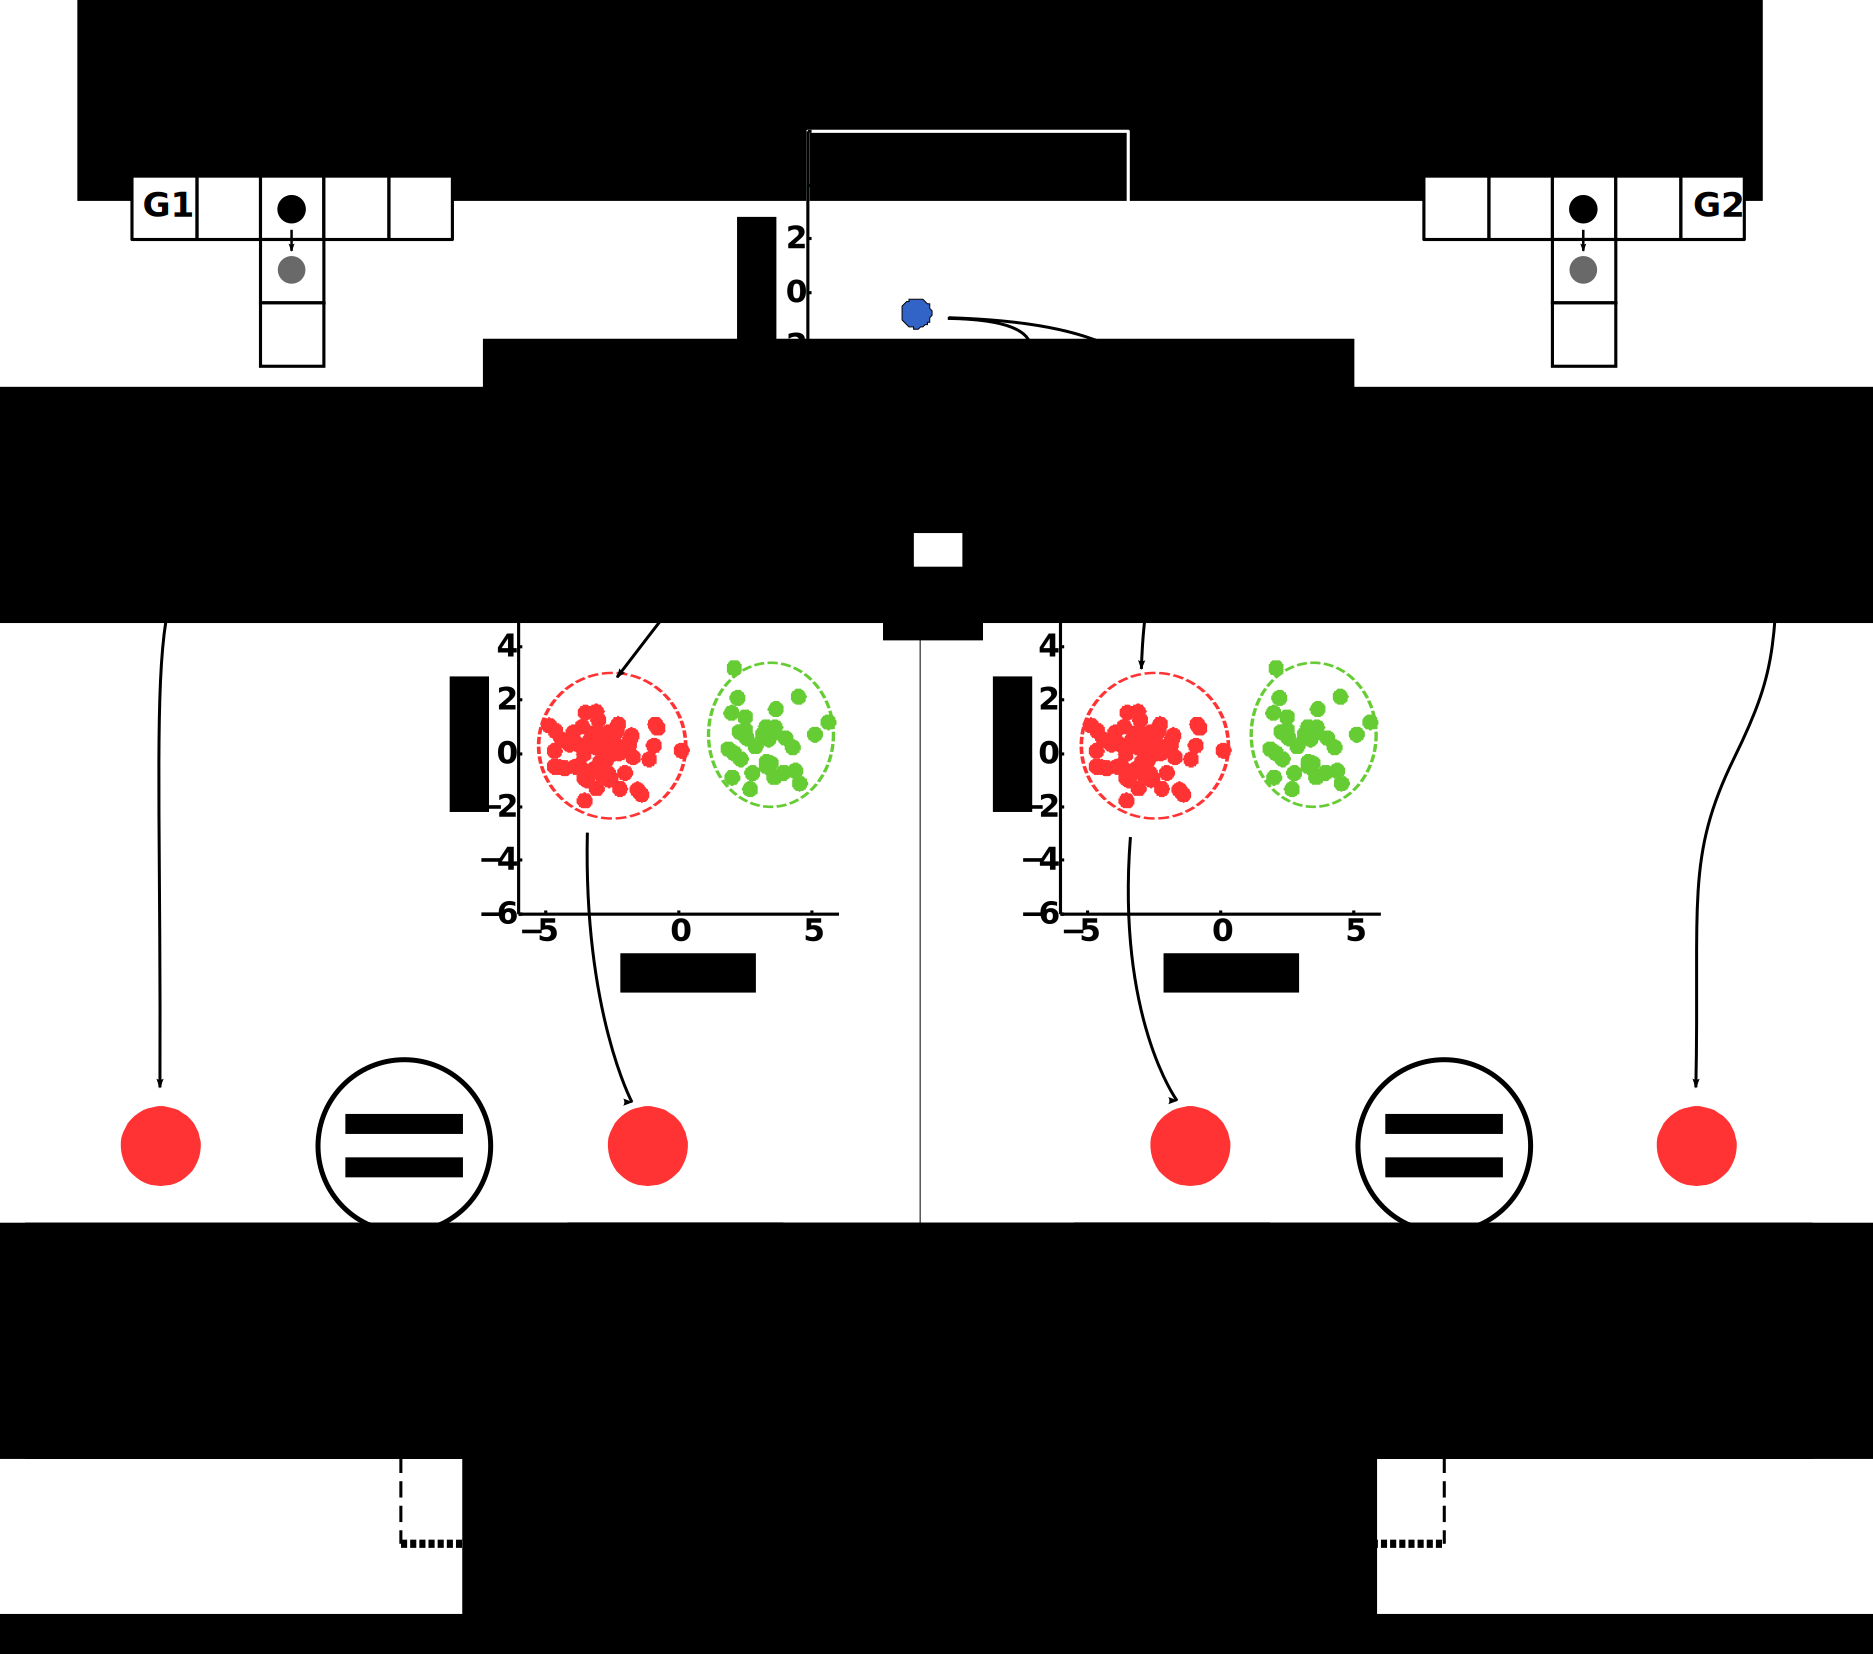
\includegraphics[width=\threeplanningwidth\columnwidth]{\visualspdf/planning/planning_up_down_expected_matched.pdf}
  \caption{Matching between expected labels and the prediction of a teaching signal sampled on the left side of the feature space for the two hypothesis if the agent performs action down in state 3 and the two hypothesis currently have a symmetric interpretation of the signals (see Figure~\ref{fig:planningupdown}). Both hypothesis agree that the label associated to a signal on the left side of the feature space match with the label predicted given the frame and the state-action pair considered. Therefore there is no uncertainty associated to this state-action pair and the agent should not select action down.}
  \label{fig:uncertaintymeaningupdownexpectedleft}
\end{figure}

However for action left, the two hypothesis disagree on whether such signals are expected or not given the state-action pair considered. As depicted in Figure~\ref{fig:uncertaintymeaningupdownunexpectedright}, when selecting action left in state 3 and if the user sends a signal in the right part of the feature space, hypothesis 1 expects a signal of meaning ``correct'', and the teacher signal is classified as being of class ``correct''. And hypothesis 2 expects a signal of meaning ``incorrect'' and the teacher signal is classified as being of class ``correct''. Therefore receiving this particular signal after taking action down in state 3 is expected for hypothesis 1 but not expected for hypothesis 2, there is high uncertainty.

\begin{figure}[!htbp]
  \centering
  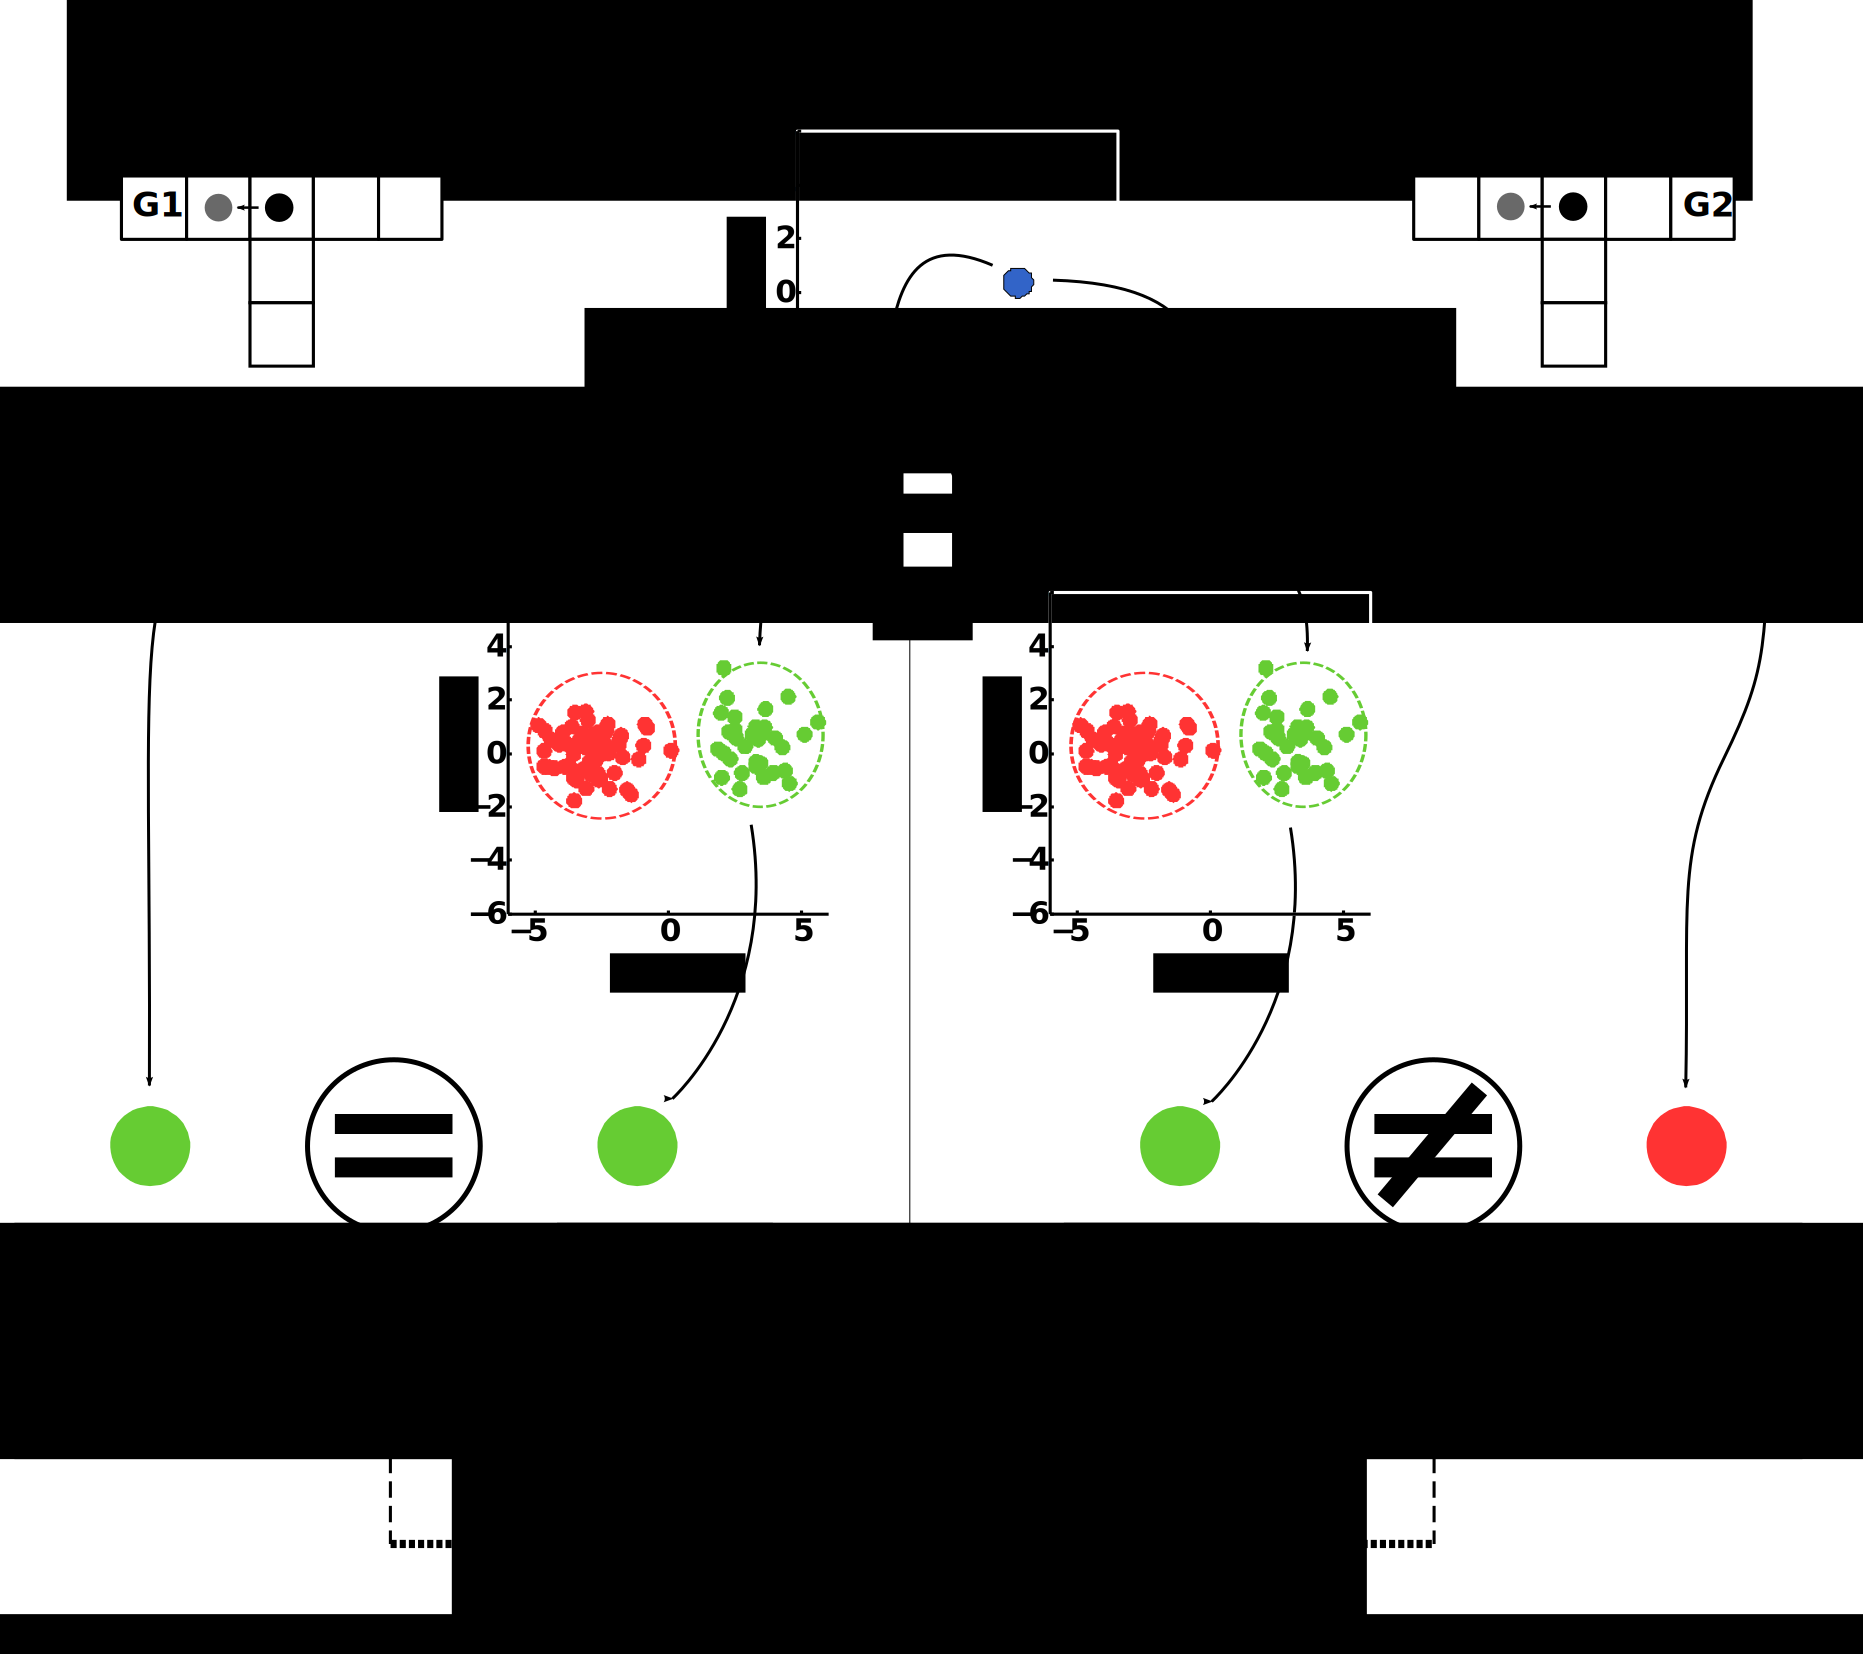
\includegraphics[width=\threeplanningwidth\columnwidth]{\visualspdf/planning/planning_up_down_unexpected_right_signal.pdf}
  \caption{Matching between expected labels and the prediction of a teaching signal sampled on the right side of the feature space for the two hypothesis if the agent performs action left in state 3 and the two hypothesis currently have a symmetric interpretation of the signals (see Figure~\ref{fig:planningupdown}). Hypothesis 1 says a signal on the right side of the feature space means ``correct'' which was expected given the interaction frame, while hypothesis 2 expected a signal meaning ``incorrect'' but classify the signal as ``correct'' which was not expected. Therefore there is high uncertainty associated to this state-action pair and the agent should better perform action left in order to disambiguate between hypothesis.}
  \label{fig:uncertaintymeaningupdownunexpectedright}
\end{figure}

Similarly, as depicted in Figure~\ref{fig:uncertaintymeaningupdownunexpectedleft}, considering a teaching signal on the left side of the feature space, if the agent performs action left in state 3, hypothesis 1 expects a signal of meaning ``incorrect'', and the teacher signal is classified as being of class ``incorrect''. And hypothesis 2 expects a signal of meaning ``incorrect'' and the teacher signal is classified as being of class ``correct''. Therefore receiving this particular signal after taking action down in state 3 is not expected for hypothesis 1 but expected for hypothesis 2, there is high uncertainty.

\begin{figure}[!htbp]
  \centering
  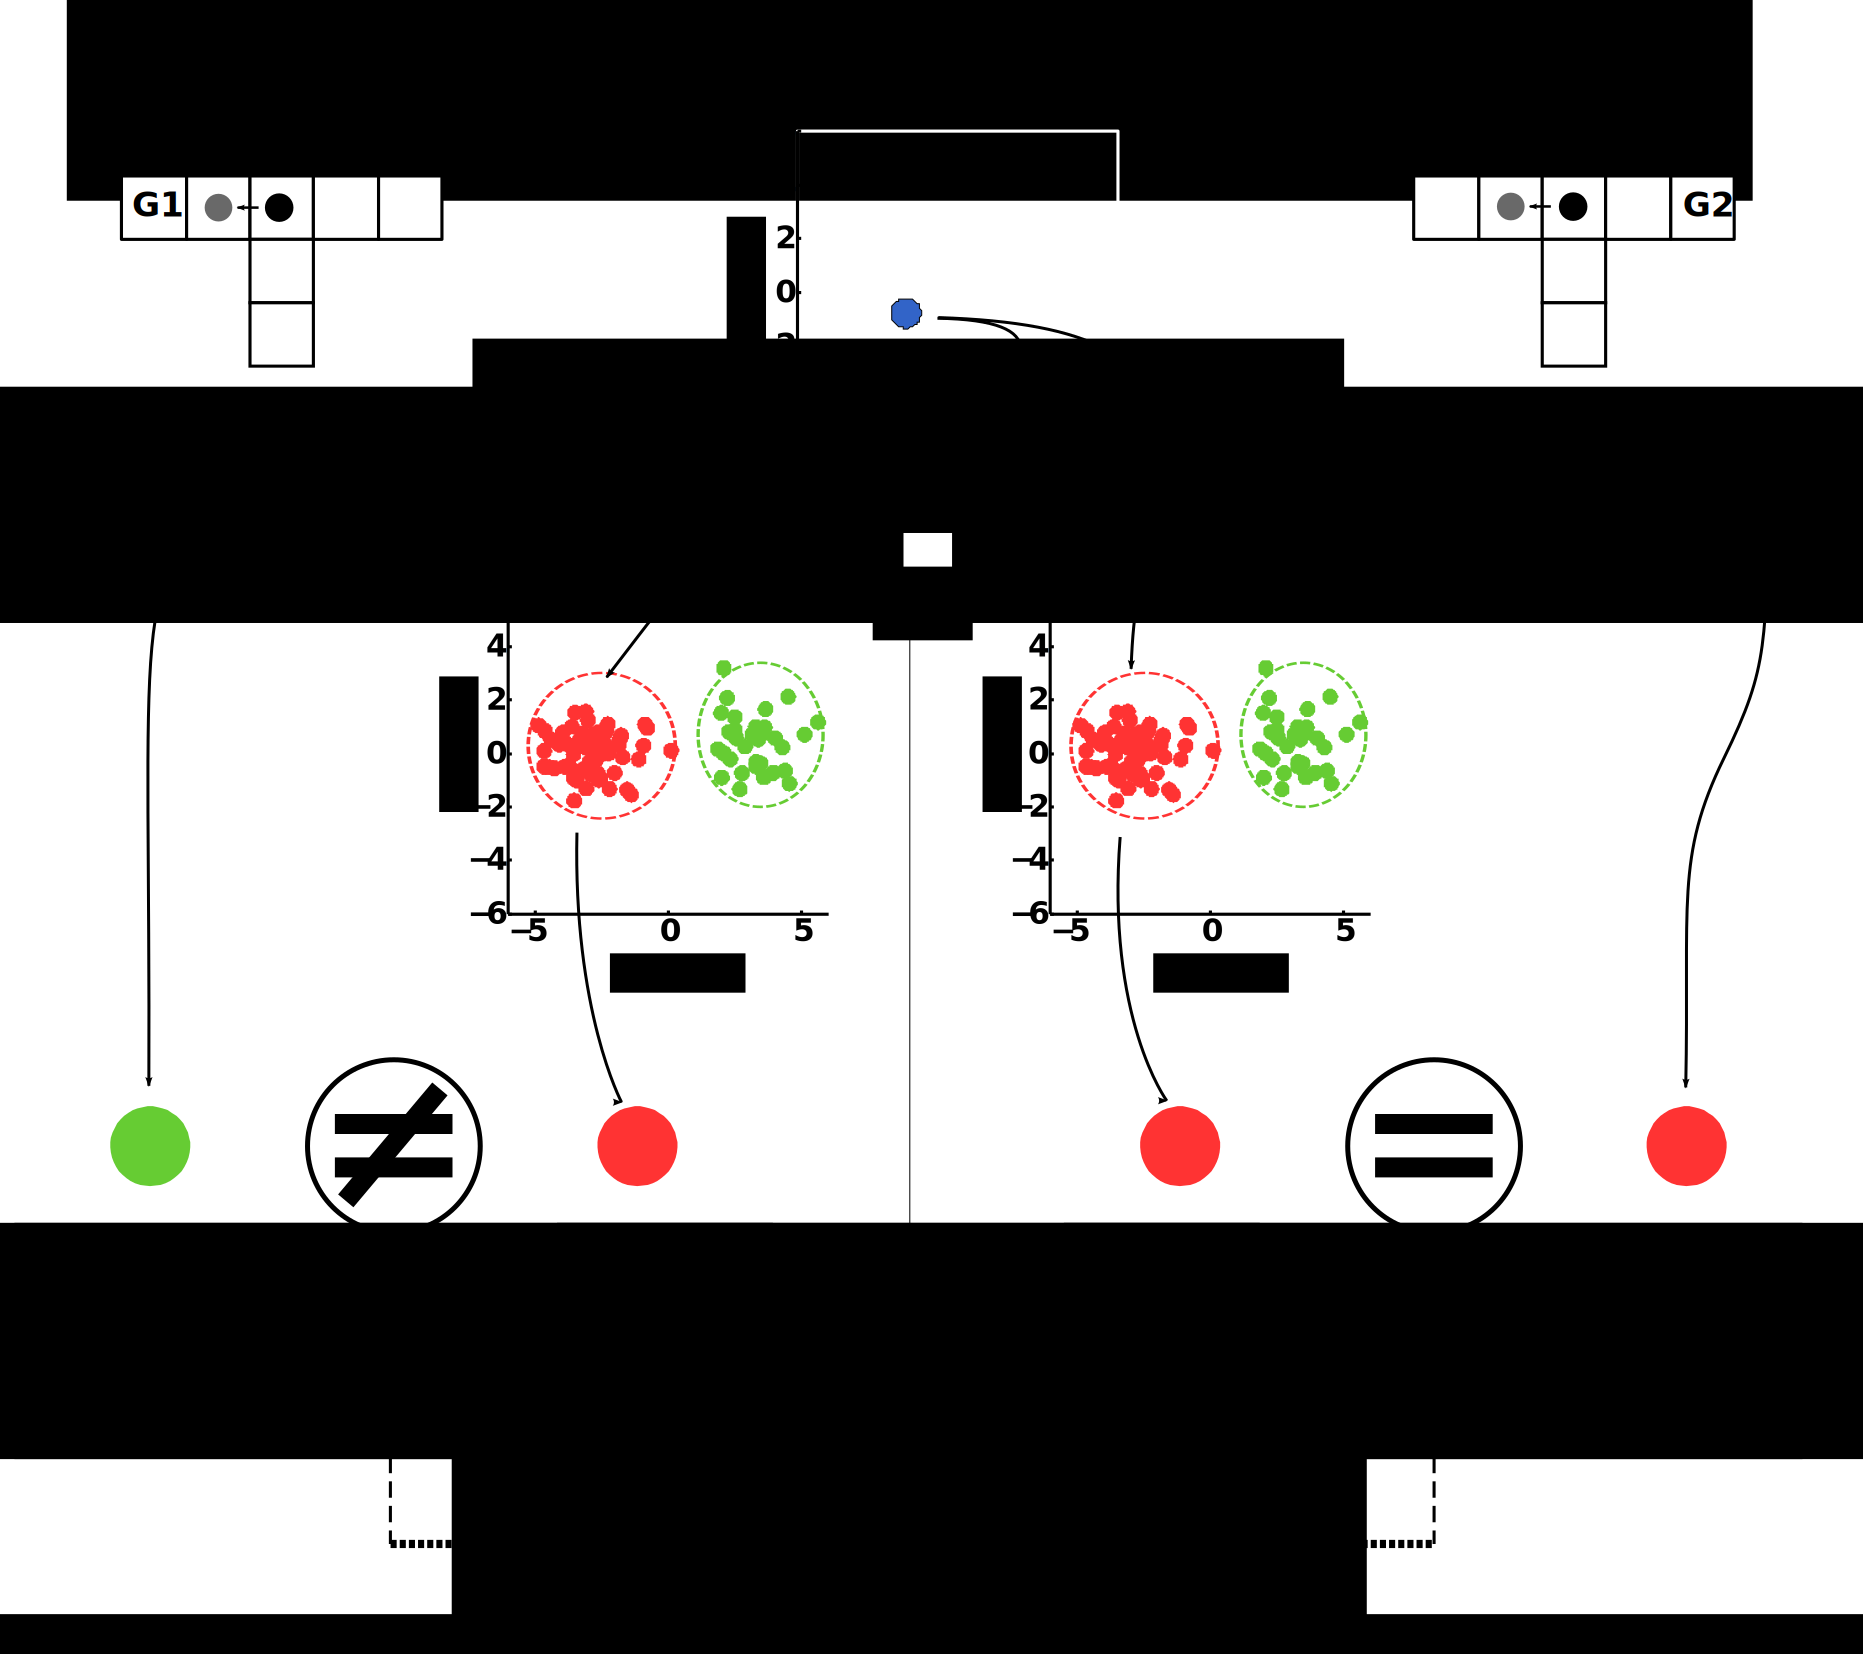
\includegraphics[width=\threeplanningwidth\columnwidth]{\visualspdf/planning/planning_up_down_unexpected_left_signal.pdf}
  \caption{Matching between expected labels and the prediction of a teaching signal sampled on the left side of the feature space for the two hypothesis if the agent performs action left in state 3 and the two hypothesis currently have a symmetric interpretation of the signals (see Figure~\ref{fig:planningupdown}). Hypothesis 1 says a signal on the left side of the feature space means ``incorrect'' which was not expected given the interaction frame, while hypothesis 2 expected a signal meaning ``incorrect'' and classify the signal as ``incorrect'' which is what was expected. Therefore there is high uncertainty associated to this state-action pair and the agent should better perform action left in order to disambiguate between hypothesis.}
  \label{fig:uncertaintymeaningupdownunexpectedleft}
\end{figure}

\subsubsection*{Equations}

To summarize, in order to estimate uncertainty between hypothesis for a given state-action pair, we can ask the system to classify some teaching signals $e$ and compute the probability that the predicted labels $l^c$ equals the expected labels $l^f$. By comparing the resulting joint probability between each hypothesis, if there is low variance there is low uncertainty. Respectively, if there is high variance, there is high uncertainty. 

This measure has the important advantage of using the same equations as the one used for computing the likelihood of each task (chapter~\ref{chapter:lfui:likelihood}). Additionally, we do not have to compute the similarity between continuous distribution, and only rely on the classifiers, that are already computed. We only need to compute the predicted labels ($l^c$) associated to the sampled signals ($e$) once per hypothesis. Then, to compute the full uncertainty map for each state and action pair, we have to compare these predicted labels with the expected labels ($l^f$) from each state-action pair and each hypothesis.

We note $J^{\xi_t}(s,a,e) = p(l^c = l^f | s, a, e, \theta_{xi_t}, \xi_t)$, which is Equation~\ref{eq:matchingoverfitting}) given the classifier $\theta_{\xi_t}$ associated to task $\xi_t$ and a particular state, action, and signal. We note $J^{\xi}(s,a,e)$ the vector $[J^{\xi_1}(s,a,e), \ldots, J^{\xi_T}(s,a,e)]$. And $W_{i}^{\xi} = [W^{\xi_1}, \ldots, W^{\xi_T}]$ the weights associated to each hypothesis. Such weights can be the one defined in Equation~\ref{eq:probapairwise} (i.e. the minimum of pairwise normalized likelihoods) or the probabilities from Equation~\ref{eq:probanormalize} (i.e. the normalized likelihoods).

The uncertainty of one state-action pair ($(s,a)$) given a signal $e$ is computed as the weighted variance of the joint probabilities:

\begin{eqnarray}
U(s,a|e) = weightedVariance(J^{\xi}(s,a,e), W^{\xi})
\label{eq:planningOneSignal}
\end{eqnarray}

The uncertainty for a state-action pair is given by:
\begin{eqnarray}
U(s,a) & = & \int_{e} U(s,a|e) p(e) de
\end{eqnarray}
which we approximate by summing values of $U(s,a|e)$ for different signals $e$:
\begin{eqnarray}
U(s,a) & \approx & \sum_{e} U(s,a|e) p(e)
\label{eq:planning}
\end{eqnarray}
with $p(e)$ assumed uniform.

Signal samples ($e$) could be sampled randomly in the all feature space. However, there is a high risk of taking non relevant samples, as well as likely practical computational problem for some classifiers. In practice, it is better to sample some signals from our past history of interaction. As the signals will be already observed by the classifiers, we may encounter overfitting problems which can be solved by using a cross validation procedure.

Our measure of uncertainty $U(s,a)$ will be higher when, for a given state-action there is a high incongruity of expectation between each hypothesis and according to the probability of each hypothesis. This measure is then used as a classical exploration bonus method. We provide an examples of planning using this method in the following of this chapter.

\transition

Interestingly the two approaches proposed generalize over other active planning methods \cite{macl09airl}, if the signal to meaning classifier is known, i.e. the same for all hypothesis, our equations reduces to the one presented in \cite{macl11simul}. For example, our first method, which relies on measuring the uncertainty on expected signals, will be equivalent to a measure on the expected meanings because all hypotheses will have identical signal's models. For our second method, all classifiers will be identical, therefore the resulting equations will no longer be dependent on signal $e$. As our uncertainty function combines uncertainty on both signal and task space, when former is known, the latter becomes the sole source of ambiguity.

\subsection{Why not building model first}

A usual question concerning Figure~\ref{fig:planningupdown}, is why don't we first select state-action pairs which lead to unequivocal interpretation of the signals? Indeed, it allows  to first build a database of known signal-label pairs. The resulting classifiers could then be use to classify further teaching signals, as in a calibration procedure.

Obviously this is not always possible, for example if we add a third hypothesis G3, that is at the bottom of the T trunk, it is not more possible to find actions leading to an unequivocal interpretation are the received signal. Neither the left and right actions (Figure~\ref{fig:planning3hyprightleft}), nor the up and down actions (Figure~\ref{fig:planning3hypupdown}) alone allow to have an unequivocal interpretation of the teaching signals. However taking all the actions and exploring the all state space still highlight hypothesis 1 (G1) has being the goal state the user as in mind (Figure~\ref{fig:planning3hyp}).

\begin{figure}[!htbp]
  \centering
  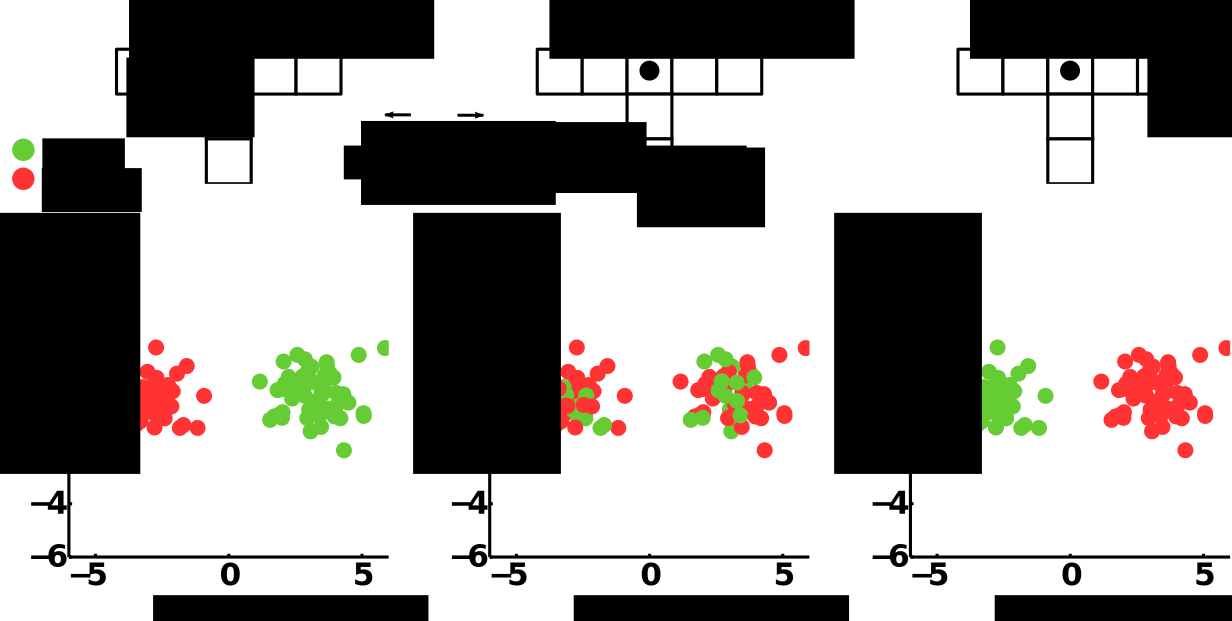
\includegraphics[width=\threetworldsize\columnwidth]{\visualspdf/planning/Tworld_feedback_3hyp_right_left.pdf}
  \caption{Interpretation hypothesis made by the agent according to G1 (left), G2 (right), and G3 (middle). The agent performs only left and right actions. The labels associated to G1 and G2 are symmetric while for G3 the labels are highly mixed. Right and left actions to not allow to have a unequivocal interpretation of signal considering those three hypothesis. However right and left actions allow to discard hypothesis G3.}
  \label{fig:planning3hyprightleft}
\end{figure}

\begin{figure}[!htbp]
  \centering
  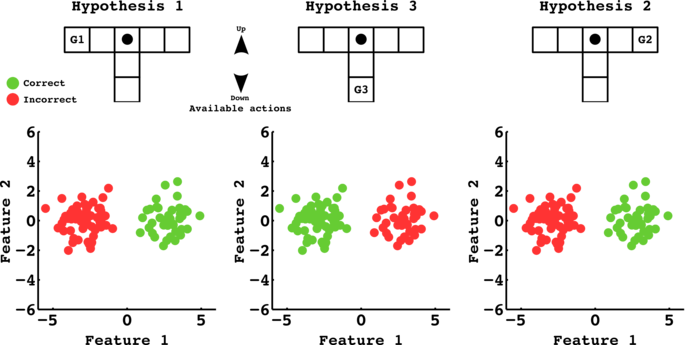
\includegraphics[width=\threetworldsize\columnwidth]{\visualspdf/planning/Tworld_feedback_3hyp_up_down_no_bump.pdf}
  \caption{Interpretation hypothesis made by the agent according to G1 (left), G2 (right), and G3 (middle). The agent performs only up and down actions. The labels associated to G1 and G2 are similar but he labels associated to G3 are symmetric. Up and down actions to not allow to have a unequivocal interpretation of signal considering those three hypothesis. Moreover u and down actions do not allow to discard any of the hypothesis.}
  \label{fig:planning3hypupdown}
\end{figure}

\begin{figure}[H]
  \centering
  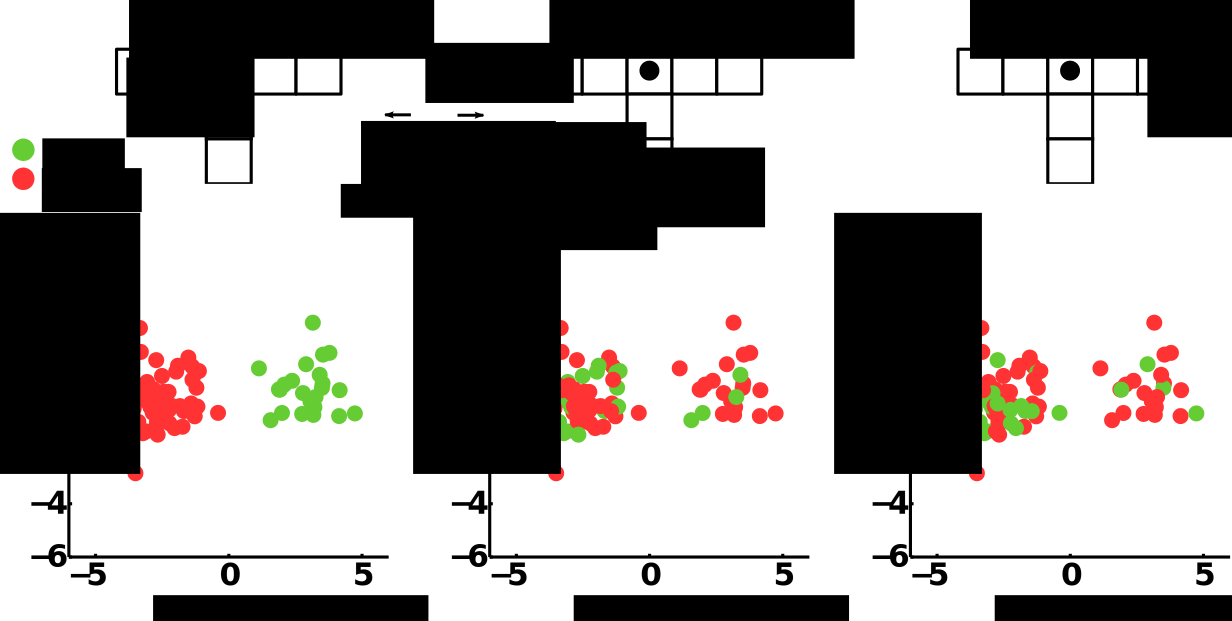
\includegraphics[width=\threetworldsize\columnwidth]{\visualspdf/planning/Tworld_feedback_3hyp.pdf}
  \caption{Interpretation hypothesis made by the agent according to G1 (left), G2 (right), and G3 (middle). The agent performs all possible actions. The labels associated to G1 are more coherent than with the spacial organization of the data than the labels associated to G2 and G3, which tells us G1 is the task the user has in mind.}
  \label{fig:planning3hyp}
\end{figure}

In all the experiments presented in this thesis, there is no state-action pairs allowing for an unequivocal interpretation of the teaching signal.

%%%%%%%%%%%%%%%%%%%%%%%%%%%%%%%%%%%%%%%%%%%%%%
%%%%%%%%%%%%%%%%%%%%%%%%%%%%%%%%%%%%%%%%%%%%%%
%%%%%%%%%%%%%%%%%%%%%%%%%%%%%%%%%%%%%%%%%%%%%%
%%%%%%%%%%%%%%%%%%%%%%%%%%%%%%%%%%%%%%%%%%%%%%
%%%%%%%%%%%%%%%%%%%%%%%%%%%%%%%%%%%%%%%%%%%%%%
\section{Method}
\label{chapter:planning:method}

In the subsequent analysis, we considerer a reaching task where an agent lives in a grid world and should learn to which square the teacher wants it to go. We considered the teacher provides feedback for the actions taken by the agent. We will use artificial dataset of different qualities and dimension to evaluate our algorithm.

% Our aim is to apply this algorithm to brain computer interaction, and we will use artificial dataset of different qualities and dimension to simulated EEG signals.

\subsection{World and Task}

We consider a 5x5 grid world, where an agent can perform five different discrete actions: move up, down, left, right, or a ``no move'' action. The user goal is to teach the agent to reach one (unknown to the agent) of the 25 discrete positions which represent the set of possible tasks. We thus consider that the agent has access to 25 different task hypotheses (one with goal location at each of the cells). We use \textit{Markov Decision Processes} (MDP) to represent the problem \cite{sutton1998reinforcement}. From a given task $\xi$, represented as a reward function, we can compute the corresponding policy $\pi_{\xi}$ using, for instance, Value Iteration \cite{sutton1998reinforcement}. We consider the user is providing feedback on the agent's actions, and use the feedback frame function as previously defined in chapter~\ref{chapter:lfui} Equation~\ref{eq:feedbackframe}.


\subsection{Simulated teaching signals}
\label{chapter:planning:artificialsignals}

We analyze our algorithm using artificial datasets. The goal of this evaluation is to analyze the feasibility of learning a task from scratch in a 5x5 grid world. The artificial dataset are composed of two classes, with 1000 examples per class. Each signal was generated by sampling from a normal distribution with a covariance matrix of diagonal 1 and mean selected randomly. The datasets were generated while varying two factors: \begin{inparaenum}[(i)] \item the dimensionality of the data, where 2, 5, 10 and 30 features were tested; and \item the quality of the dataset, measured in terms of the ten-fold accuracy the classifier would obtain. \end{inparaenum} We exemplify datasets of different qualities in Figure~\ref{fig:datasetsquality}.

\begin{figure}[!htbp]
  \centering
      \includegraphics[width=\columnwidth]{\visualspdf/worlds_and_datasets/dataset_qualities.pdf}
      \caption{Artificial datasets generated by sampling from normal distributions with a covariance matrix of diagonal 1 and means selected randomly. From left to right, we show datasets of increasing quality as measured by a 10 fold cross-validation train-test procedure using a Gaussian classifier.}
    \label{fig:datasetsquality}
\end{figure}

\subsection{Signal properties and classifier}

% We aim at applying this algorithm to error-related potentials (ErrPs) for EEG-based BCI applications. These signals are generated in the user's brain after s/he assesses actions performed by an external agent \cite{chavarriaga2010learning}, where correct and erroneous assessments will elicit different brain signals. Past approaches have already demonstrated that these signals can be classified online with accuracies of around 80\% and translated into binary feedback, thanks to a prior calibration session that lasts for 30-40 minutes \cite{chavarriaga2010learning, iturrate2013task}.

% Following the literature \cite{lotte2007review,blankertz2010single}, w

We rely on Gaussian classifiers and model the signals using independent multivariate normal distributions for each class, $\mathcal{N}(\mu_c, \Sigma_c), \mathcal{N}(\mu_w, \Sigma_w)$. With $\theta$ the set of parameters $\{\mu_c, \Sigma_c,\mu_w, \Sigma_w\}$. Given the high dimensionality of some datasets we also need to regularize. For this we apply shrinkage to the covariance matrix ($\lambda = 0.5$) and compute the value of the marginal pdf function using a noninformative (Jeffrey's) prior [\cite{gelman2003bayesian}, p88]:

\begin{eqnarray}
p(e|l, \theta) & = & t_{n-d}(e | \mu_l,\frac{\Sigma_l (n+1)}{n(n-d)})
\label{eq:prior}
\end{eqnarray}

where $\theta$ represents the ML estimates (mean $\mu_l$ and covariance $\Sigma_l$ for each class $l$) required to estimate the marginal under the Jeffreys prior, $n$ is the number of signals, and $d$ is the dimensionality of a signal feature vector.

Finally to compute the probability of a label given a signal, we use the bayes rules as follows: 
%
\begin{eqnarray}
    p(l = l_i|e,\theta) &=& \frac{p(e|l = l_i, \theta)p(l = l_i)}{\sum_{k = 1,\ldots, L}{p(e|l = l_k,\theta)p(l = l_k)}}\nonumber \\
    &=& \frac{p(e|l=l_i, \theta)}{\sum_{k = 1,\ldots, L} p(e|l=l_k)} \nonumber
\end{eqnarray}
%
As we do not have a priori knowledge on the user intended meaning, we assume all labels are equiprobables, i.e. $\forall k,~p(l = l_k) = \frac{1}{L}$.

\subsection{Task Achievement}

We use Equation~\ref{eq:matchingfiltercrossvalidation} to compute the likelihood of each task using a 10 fold cross-validation to compute the confusion matrix. It implies we train 250 classifiers at each iteration. To compute the probability of each task, we will rely on the minimum of pairwise normalized likelihood measure as defined in Equation~\ref{eq:probapairwise}.

A task is considered completed when the confidence level $\beta$ as been reached for this task and the agent is located at the task associated goal state. If the corresponding state is the one intended by the user, it is a success. Whatever the success or failure of the first task, the user selects a new task, i.e. a new goal state, randomly. The agent resets the task likelihoods, propagates the previous task labels to all hypothesis, and the teaching process starts again. At no point the agent has access to a measure of its performance, it can only refer to the unlabeled feedback signals from the user.

\subsection{Evaluation scenarios}

Using our artificial datasets, three different evaluations are performed: \begin{inparaenum}[(i)] \item the performance of our proposed planning strategy versus a) random action selection, b) greedy action selection, and c) a task-only uncertainty based method; \item the time required by the agent to complete the first task (i.e. to reach the first target with confidence), and \item the number of tasks that can be completed in 500 iterations. \end{inparaenum}

\subsection{Settings}

We used $\alpha = 0.1$, $\beta = 0.9$. For dataset of dimension $d$, we started computing likelihoods after $d+10$ steps as equation \ref{eq:prior} requires at least $d+1$ samples and to allow for cross validation. For the planning (Eq. \ref{eq:planning}) we sample randomly 20 signals from $D_M$.

%%%%%%%%%%%%%%%%%%%%%%%%%%%%%%%%%%%%%%%%%%%%%%
%%%%%%%%%%%%%%%%%%%%%%%%%%%%%%%%%%%%%%%%%%%%%%
%%%%%%%%%%%%%%%%%%%%%%%%%%%%%%%%%%%%%%%%%%%%%%
%%%%%%%%%%%%%%%%%%%%%%%%%%%%%%%%%%%%%%%%%%%%%%
%%%%%%%%%%%%%%%%%%%%%%%%%%%%%%%%%%%%%%%%%%%%%%
\section{Illustration of the grid world scenario}
\label{chapter:planning:gridworld}

We illustrate in Figure~\ref{fig:planning:gridworldfeedback}, a smaller 3x3 grid world example and the results of the hypothetic labeling process. The teacher is providing feedback with respect to hypothesis 1. The labeling process for hypothesis 1 is the more coherent. We note that hypothesis 9 has symmetric properties with hypothesis 1 but the use of the ``no move'' action allows to break that symmetry.

\begin{figure}[!htbp]
  \centering
  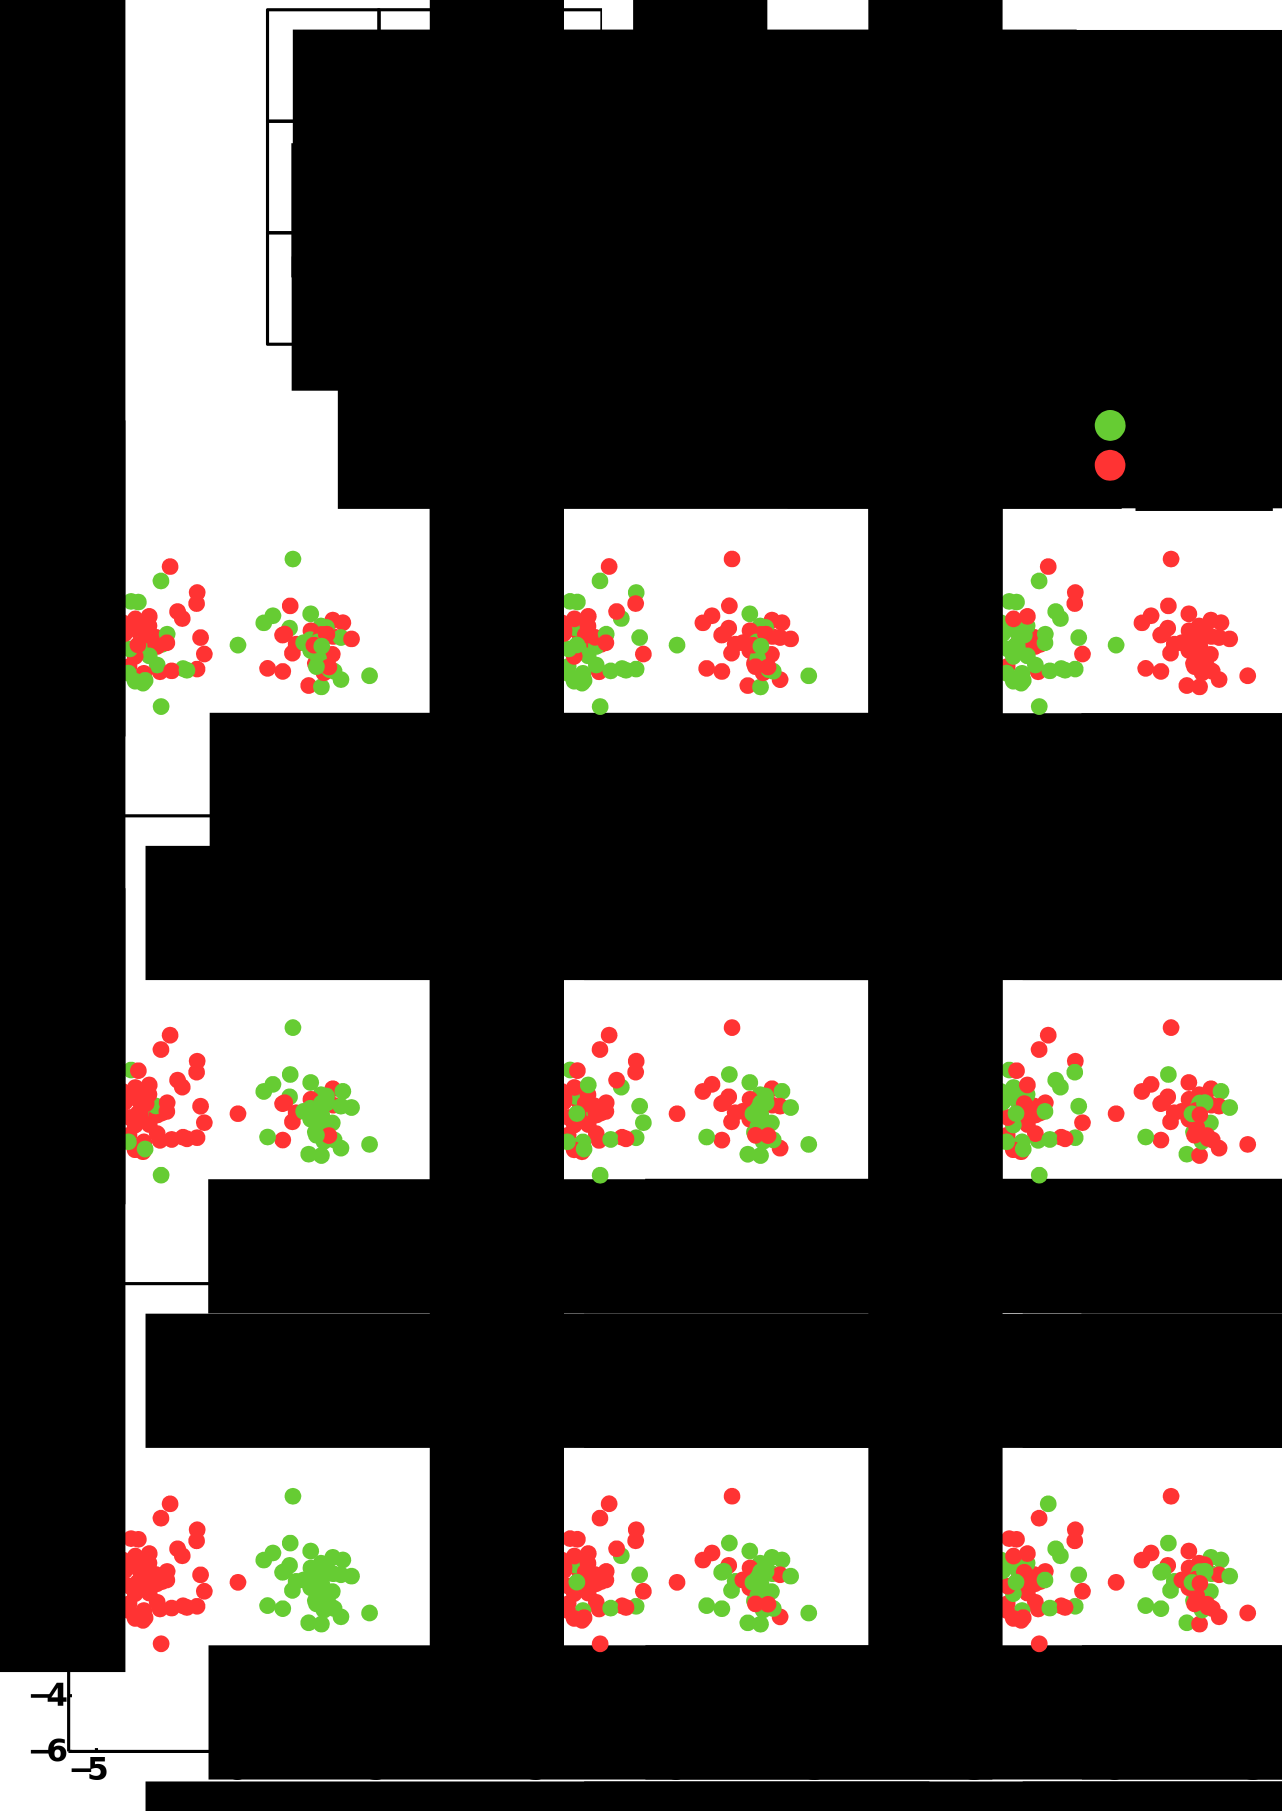
\includegraphics[width=\columnwidth]{\visualspdf/gridworld/gridworld_feedback.pdf}
  \caption{A schematic view of a 3x3 grid world scenario. There is nine possible hypotheses and the agent is acting randomly for this example. We show the results of the labeling process considering the feedback frame. The teacher is providing feedback with respect to hypothesis 1. The labeling process for hypothesis 1 is more coherent with the spacial organization of the data which indicates it is the one taught by the user. Hypothesis 9 has symmetric properties with hypothesis 1 but the use of the ``no move'' action allows to break that symmetry.}
  \label{fig:planning:gridworldfeedback}
\end{figure}

%%%%%%%%%%%%%%%%%%%%%%%%%%%%%%%%%%%%%%%%%%%%%%
%%%%%%%%%%%%%%%%%%%%%%%%%%%%%%%%%%%%%%%%%%%%%%
%%%%%%%%%%%%%%%%%%%%%%%%%%%%%%%%%%%%%%%%%%%%%%
%%%%%%%%%%%%%%%%%%%%%%%%%%%%%%%%%%%%%%%%%%%%%%
%%%%%%%%%%%%%%%%%%%%%%%%%%%%%%%%%%%%%%%%%%%%%%
\section{Results}
\label{chapter:planning:results}

In the following, we present most of the results in terms of the quality of the dataset, measured as the ten-fold classification accuracy that a calibrated signal classifier would obtain. Each simulation was run 100 times using different sampled datasets, and their associated box plots were computed. For each boxplot, colored bars show the interquartile range (between 25th and 75th percentile). The median and the mean are marked as a horizontal line and a colored dot respectively. The two whiskers show the 5th and 95th percentiles, black crosses are outliers. 

We first study the impact of the uncertainty based exploration approach proposed in this chapter. We then evaluate the performance and robustness of our algorithm with respect to the dimension and the quality of the datasets.

\subsection{Planning methods}

Figure~\ref{fig:artificialplanning} compares the number of steps (with maximum values of 500 steps) needed to reach the first task with confidence using different planning methods. Following the most probable task (i.e. going greedy) does not allow the system to explore sufficiently. The planning method proposed in this chapter leads the system towards state-action pairs that discriminates hypotheses faster. Furthermore, our planning method performs better than assessing uncertainty on the meaning space only. Given these results, the remaining of this section will only consider our planning method.

\begin{figure}[!htbp]
  \centering
      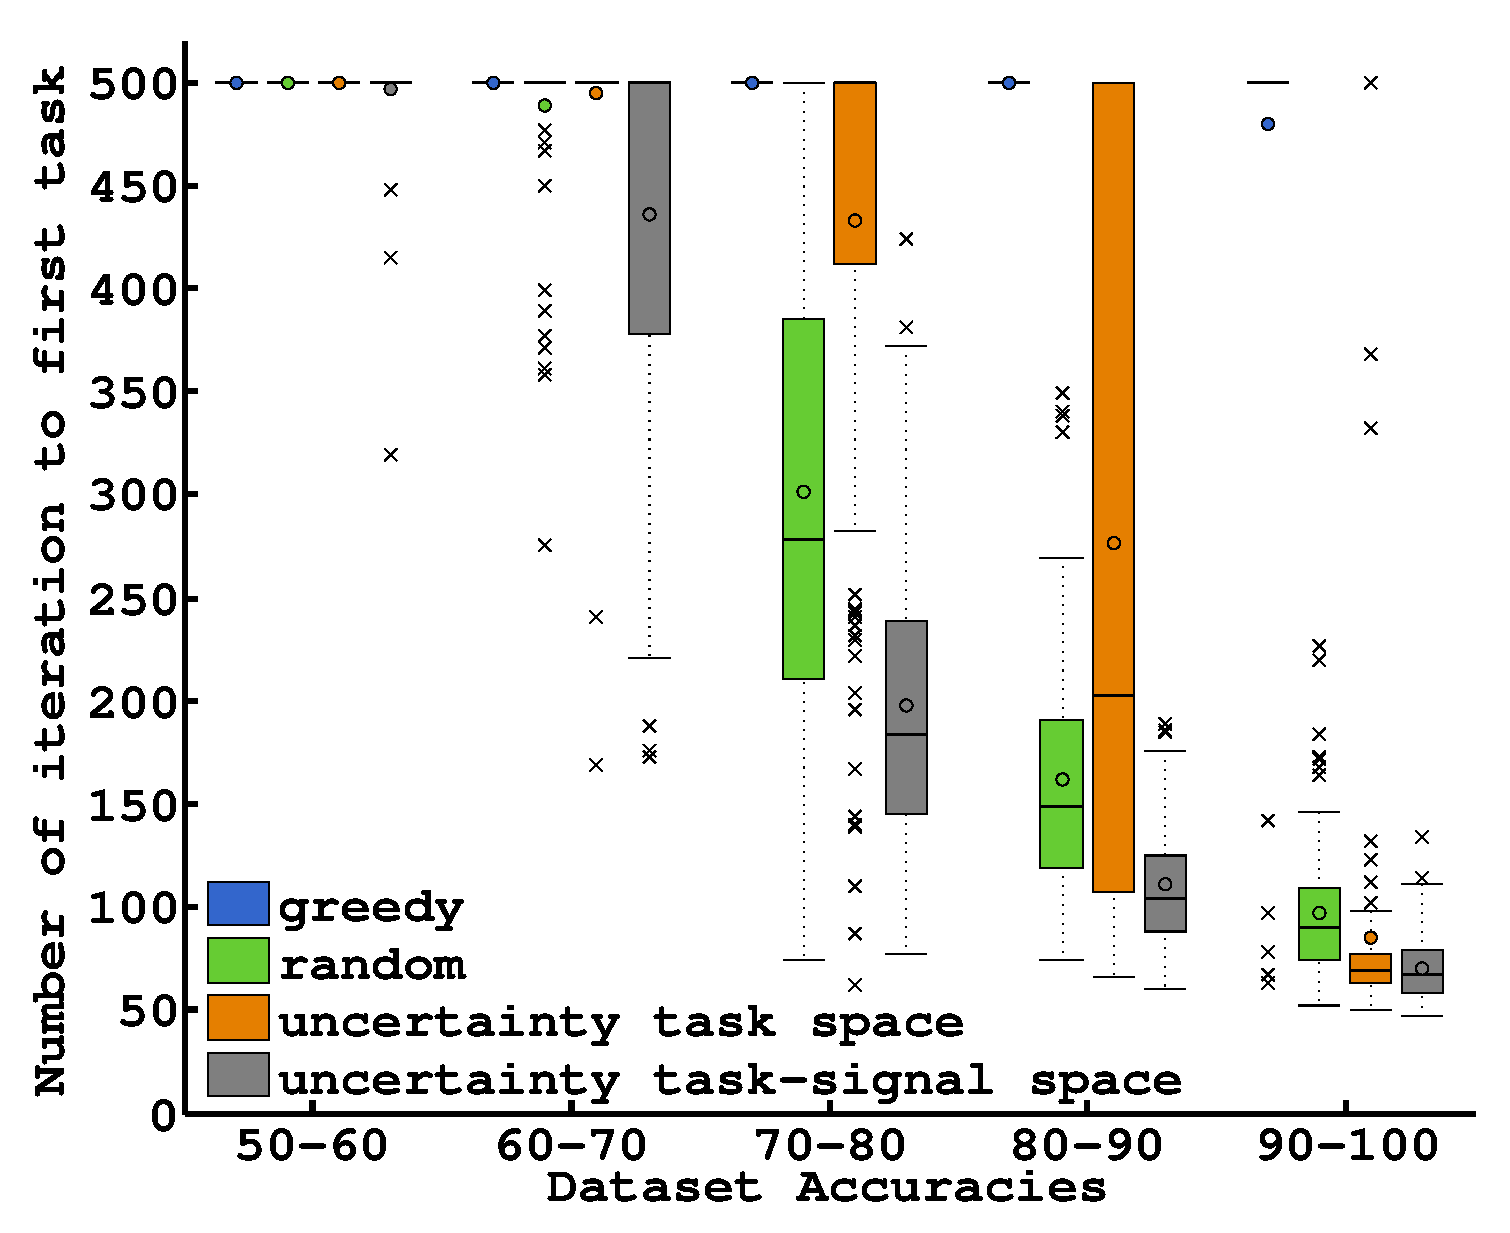
\includegraphics[width=\plotsize\columnwidth]{\imgpath/plot_artificial_planning.eps}
      \caption{Number of steps to complete the first task, comparison of different exploration methods with 30 dimensional artificial data. When learning from scratch, planning upon both the task and the signal to meaning mapping uncertainty performs better than relying only on the uncertainty about the task. Greedy action selection rarely disambiguates between hypothesis.}
    \label{fig:artificialplanning}
\end{figure}

As explained in section~\ref{chapter:planning:how}, the machine needs to collect two types of information, some about the true underlying model (Fig.~\ref{fig:planningupdown}) and some to differentiate between hypotheses (Fig.~\ref{fig:planningrightleft}). The properties of the grid world make the random strategy quite efficient at collecting those two types of information. The differences between our active planning method and a random exploration should be sharper when navigating a complex maze.

We present a small study on how different world properties affect the learning efficiency in chapter~\ref{chapter:limitations:wordlproperties}.

Finally, we note that all planning methods were switched to pure exploitation (greedy) once the confidence level was reached. Therefore the performance in Figure~\ref{fig:artificialplanning} compares the ability of the different methods to discriminate between different task hypotheses, not their ability to solve the task itself.

\subsection{Dimensionality}

Figure~\ref{fig:firstArtificial} compares the number of steps (with maximum values of 500 steps) needed to reach the first task with confidence when learning from scratch considering different dimensionality of datasets. The convergence speed is only slightly affected by the features dimensionality. On the other hand, the dataset quality (measured in terms of its associated ten-fold accuracy) is the main cause of performances decay. Furthermore, for these datasets with accuracies between $50\%$ and $60\%$, the system is not able to identify a task with confidence after 500 steps. This is the expected behavior as for such dataset (see Figure~\ref{fig:datasetsquality} left), none of the hypothesis is able to find a classifier of good enough accuracy and should therefore not take any decision.

\begin{figure}[!htbp]
  \centering
      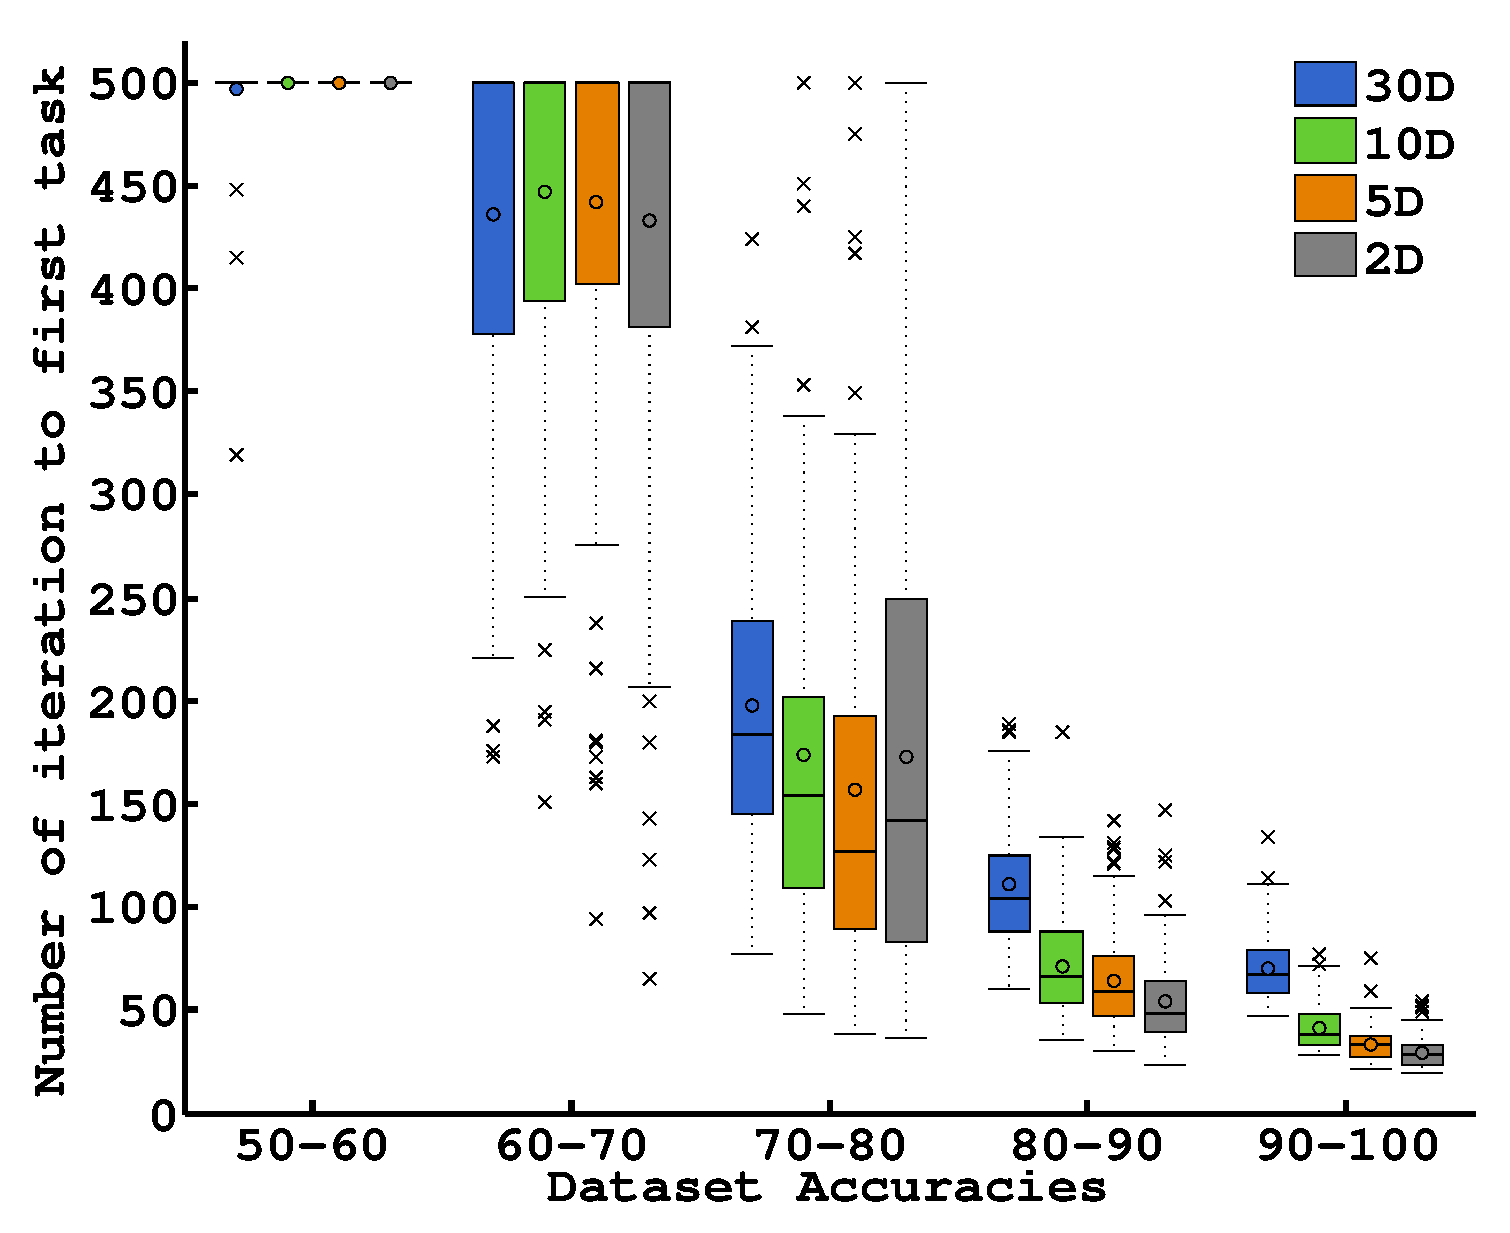
\includegraphics[width=\plotsize\columnwidth]{\imgpath/plot_artificial_firstconf.eps}
      \caption{Number of steps to complete the first task using artificial data. For datasets of low quality, i.e. under 60 percent accuracy, the confidence threshold cannot be reached in 500 steps. The datasets' quality, more than their dimensionality, impacts the learning time.}
      \label{fig:firstArtificial}
\end{figure} 

\subsection{Reuse}

Once the first task is completed, a new one is selected randomly. Figure~\ref{fig:nCorrectArtificial} compares the number of tasks that can be achieved in 500 steps. As expected, the lower the quality of the data, the less number of tasks can be completed. With dataset of accuracies higher than $90\%$ we can achieve more than 30 tasks on average.

\begin{figure}[!htbp]
    \centering
    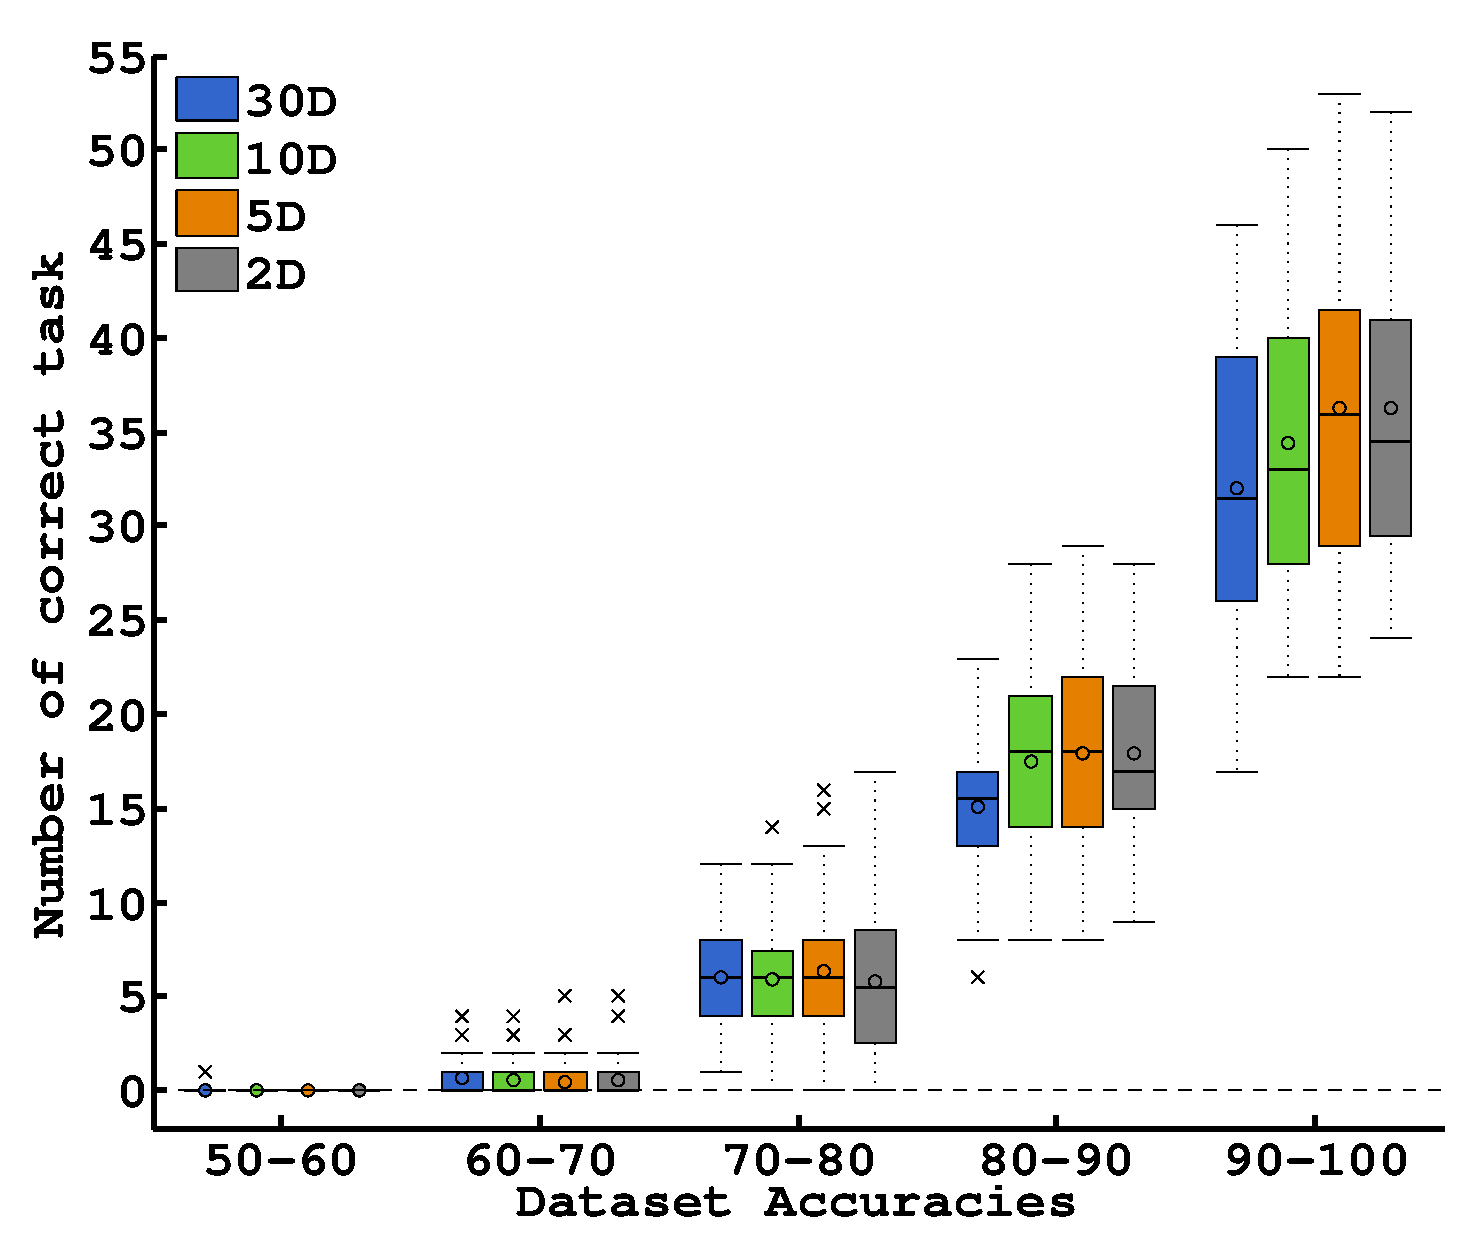
\includegraphics[width=\plotsize\columnwidth]{\imgpath/plot_artificial_nCorrect.eps}
    \caption{Number of tasks correctly achieved in 500 steps using artificial data. Quality of datasets impacts the number of tasks identified in 500 steps because more evidence should be collected to reach the confidence threshold.}
    \label{fig:nCorrectArtificial}
\end{figure} 

Importantly, our algorithm makes very few mistakes when identifying the first task. We reported only 9 erroneous estimations across all simulated experiments (5 in the 70-80 group and 4 in the 80-90 group).

\section{Discussion}

In this chapter, we presented a planning method allowing to reduce the number of iterations needed to identify the correct task from unlabeled teaching signals. This method was based on assigning an uncertainty value to each state-action pair. By asking the agent to look for the most uncertain state-action pair, it can collect more useful data to disambiguate faster between the hypotheses. We identified two sources of uncertainty, one coming from the task and the other coming from the signal model associated to each task hypothesis. We presented two methods to measure this uncertainty. The first method measures the uncertainty on the expected signals between each hypothesis. The second method measures uncertainty on the meaning space by making hypothesis on future observed signals.

We want to apply this algorithm to a more concrete scenario with real users. In next chapter, we present a brain computer interaction scenario following the reaching task presented in this section. But instead of using artificial data, we will investigate own our algorithm scale to brain signals, first in simulation and then during online experiments with real subjects.

% The application of this work to BCI is a joint collaboration with I{\~n}aki Iturrate and Luis Montesano.
